\documentclass[output=paper,colorlinks,citecolor=brown]{langscibook}
\ChapterDOI{10.5281/zenodo.21237020}
\author{Iris Tanza-Kamil\orcid{}\affiliation{The Hebrew University of Jerusalem}}
%\ORCIDs{}

\title{Deriving the Akkadian Stative: A deadjectival verb?}

\abstract{Recent studies on the Akkadian Stative conjugation have defended its verbal nature \citep{kouwenberg_nouns_2000,carver_akkadian_2016,kamil2023stative}, arguing against approaches that have treated it as a nominal element \citep{huehnergard_stative_1987,buccellati_state_1988}. The nominal argument stems from the Stative's diachronic origin as a verbal adjective (VA); synchronically, it is thus often treated as a denominal/deadjectival verb \citep{kouwenberg_nouns_2000}. This present contribution argues for two separate trajectories of Stative derivation: Primary Statives, i.e., Statives whose base is a VA, are derived deradically, while secondary Statives, i.e., Statives whose base is a nominal or adjectival stem, are derived denominally or deadjectivally. I motivate these different trajectories based on mismatches observed between Statives and VAs derived from the same \textsc{lexical root}, pertaining to 1) the argument predicated by either Stative or VA, and 2) the resultative readings of Statives vis-à-vis VAs. First, I show that Experiencer-subject transitives feature mismatches in argument predication: While their Statives predicate the Experiencer-subject, their VAs predicate the Theme-object. Secondly, I motivate the resultative reading of Statives as a consequence of their derivation: Primary Statives inherit their change-of-state event directly from the \textsc{root}. Secondary Statives require external syntactic or pragmatic cues to achieve resultative readings.
}


\IfFileExists{../localcommands.tex}{
   \addbibresource{../localbibliography.bib}
   \usepackage{tabularx,multicol}
\usepackage{url}
\urlstyle{same}

 
\usepackage{langsci-optional}
\usepackage{langsci-lgr}
\usepackage{langsci-gb4e}
\usepackage[linguistics,edges]{forest}
\usepackage{tikz-qtree}
\usetikzlibrary{positioning}
\usetikzlibrary{patterns.meta}
\usepackage{multirow}
\usepackage{pgfplots}
\usepackage{setspace}
\usepackage{amsmath,stackengine}
% \usepackage{fontspec}
% \usepackage{tipa} % TIPA is banned
\usepackage{langsci-textipa}
\usepackage{langsci-branding}
\usepackage{longtable}
\usepackage{tabto}

\usepackage{enumitem}

%\usepackage{lscape} %Querformat chapter 4

   % \newcommand*{\orcid}{}


\makeatletter
\let\thetitle\@title
\let\theauthor\@author
\makeatother

\newcommand{\togglepaper}[1][0]{
   \bibliography{../localbibliography}
   \papernote{\scriptsize\normalfont
     \theauthor.
     \titleTemp.
     To appear in:
    Laura Grestenberger, Viktoria Reiter \& Melanie Malzahn (eds.).
    \emph{Deadjectival verb formation in Indo-European and beyond}.
     Berlin: Language Science Press. [preliminary page numbering]
   }
   \pagenumbering{roman}
   \setcounter{chapter}{#1}
   \addtocounter{chapter}{-1}
}

\newbool{bookcompile}
\booltrue{bookcompile}
\newcommand{\bookorchapter}[2]{\ifbool{bookcompile}{#1}{#2}}

%Sonderzeichen
%idg palatales k
\newcommand{\kinvbreve}{k\raisebox{0.6ex}{\hspace{-0.05em}\char"0311}}

\newcommand{\jac}{%
  \textit{\char"0237}% italic dotless j (ȷ)
  \hspace{-0.01em}% fine-tune horizontal spacing
  \raisebox{0.01ex}{\char"0301}% raised combining acute
}

%Baltic circumflex l
\newcommand\ltilded{%
\hspace{-0.2em}%
  \stackon[-1.5pt]{l}{\smash{\kern0.2em\~{}}}%
  \hspace{-0.2em}%
}

%Slav. wedge+ double acute
\newcommand{\HighH}[1]{%
    \stackon[-1.2ex]{#1}{\kern0.1em\H{}\kern-0.1em}%
}

%Lith dot tilde VICKY diese b.-sl. Sonderzeichen BRINGEN MICH UM!!
\newcommand{\tildedot}[1]{%
    \ensurestackMath{%
        \stackon[-0.27ex]{% Tilde layer 
            \stackon[-0.15ex]{% Dot layer 
                #1%
            }{\hspace{0.1em}\cdot\hspace{-0.13em}}%
        }{\hspace{0.1em}\text{\~{}}\hspace{-0.13em}%
    }%
}}

%Lith dot acute
\newcommand{\dotacute}[1]{%
    \ensurestackMath{%
        \stackon[-1.1ex]{% acute layer 
            \stackon[-0.15ex]{% Dot layer 
                #1%
            }{\hspace{0.1em}\cdot\hspace{-0.12em}}%
        }{\hspace{0.1em}\text{\'{}}\hspace{-0.12em}%
    }%
}}



% \setlength{\emergencystretch}{2pt} 

 \pgfplotsset{compat=1.18}


\defcitealias{AbB_1}{AbB 1}
\defcitealias{AbB_7}{AbB 7}
\defcitealias{ABL_1}{ABL 1}
\defcitealias{Vries1977}{AEW}
\defcitealias{ALEW}{ALEW}
\defcitealias{AnGr}{AnGr}
\defcitealias{ARM_1}{ARM 1}
\defcitealias{BT}{BT}
\defcitealias{black_concise_2000}{CDA}
\defcitealias{CHD}{CHD}
\defcitealias{CT28}{CT 28}
\defcitealias{CT34}{CT 34}
\defcitealias{CT39}{CT 39}
\defcitealias{Cleasby1874}{CV}
\defcitealias{Beekes2010}{EDG}
\defcitealias{eDiAna}{eDiAna}
\defcitealias{eDIL}{eDIL}
\defcitealias{EDL}{EDL}
\defcitealias{Kroonen2013}{EDPG}
\defcitealias{ESJS}{ESJS}
\defcitealias{EVP}{EVP}
\defcitealias{EWA1988}{EWA}
\defcitealias{EWAI}{EWAia I}
\defcitealias{EWAII}{EWAia II}
\defcitealias{EWGP}{EWGP}
\defcitealias{GDLI1961}{GDLI}
\defcitealias{GPC}{GPC}
\defcitealias{GRADIT1999}{GRADIT}
\defcitealias{HW}{HW}
\defcitealias{IEW}{IEW}
\defcitealias{KAH_2}{KAH 2}
\defcitealias{KAR_1}{KAR 1}
\defcitealias{KAR_2}{KAR 2}
\defcitealias{KEWA}{KEWA}
\defcitealias{Labat_TDP}{Labat TDP}
\defcitealias{lambert_BWL}{Lambert BWL}
\defcitealias{LEIA}{LEIA}
\defcitealias{Rix2001}{LIV\textsuperscript{2}}
\defcitealias{LIVaddenda}{LIV\textsuperscript{2} {A}ddenda}
\defcitealias{LKG1971}{LKG}
\defcitealias{LKZ}{LKŽ}
\defcitealias{LP}{LP}
\defcitealias{MhdGr}{MhdGr}
\defcitealias{MLLVG1959}{MLLVG}
\defcitealias{NIL}{NIL}
\defcitealias{OgnS}{OgnS}
\defcitealias{ONP}{ONP}
\defcitealias{RIMA_2}{RIMA 2}
\defcitealias{TIM_2}{TIM 2}
\defcitealias{WAP}{WAP}
\defcitealias{YOS_2}{YOS 2}






\newindex{wan}{wdx}{wnd}{Form index}
\newcommand{\iw}[2]{\index[wan]{#1!{#2}\xspace}}
\newcommand{\iwi}[3][]{\index[wan]{#2!{#3}\xspace#1}{#3}}
\newcommand{\iwit}[3][]{\rule{0pt}{0pt}#1\index[wan]{#2!{#3}}{#3}}


\newindex{van}{vdx}{vnd}{Form index}
\newindex{ban}{bdx}{bnd}{Book index}

% \newcommand{\iw}[3][]{\index[wan]{#2!\textit{#3}}}


% \providecommand{\iwi}[3][]{\iw{#3}\textit{#3}}


\newcommand{\indexnote}[1]{{\footnotesize\sffamily\raggedright\normalfont\color{gray}#1}}

   %% hyphenation points for line breaks
%% Normally, automatic hyphenation in LaTeX is very good
%% If a word is mis-hyphenated, add it to this file
%%
%% add information to TeX file before \begin{document} with:
%% %% hyphenation points for line breaks
%% Normally, automatic hyphenation in LaTeX is very good
%% If a word is mis-hyphenated, add it to this file
%%
%% add information to TeX file before \begin{document} with:
%% %% hyphenation points for line breaks
%% Normally, automatic hyphenation in LaTeX is very good
%% If a word is mis-hyphenated, add it to this file
%%
%% add information to TeX file before \begin{document} with:
%% \include{localhyphenation}
\hyphenation{
    par-a-digm non-de-adj-ect-iv-al -pre-sent -pre-sents for-ma-tion-al in-do-ger-ma-ni-sche in-do-ger-ma-ni-schen Rei-chert Rei-ter dia-chrony ety-mo-lo-gi-sches Ost-ger-ma-ni-schen ger-ma-ni-schen alt-in-di-schen mor-pho-lo-gi-scher Alt-indo-ari-sch-en lexico-graphy Schrij-ver
}
% aktuell in Bibliographie: stud-ies, histor-ical Soci-età
\hyphenation{
    par-a-digm non-de-adj-ect-iv-al -pre-sent -pre-sents for-ma-tion-al in-do-ger-ma-ni-sche in-do-ger-ma-ni-schen Rei-chert Rei-ter dia-chrony ety-mo-lo-gi-sches Ost-ger-ma-ni-schen ger-ma-ni-schen alt-in-di-schen mor-pho-lo-gi-scher Alt-indo-ari-sch-en lexico-graphy Schrij-ver
}
% aktuell in Bibliographie: stud-ies, histor-ical Soci-età
\hyphenation{
    par-a-digm non-de-adj-ect-iv-al -pre-sent -pre-sents for-ma-tion-al in-do-ger-ma-ni-sche in-do-ger-ma-ni-schen Rei-chert Rei-ter dia-chrony ety-mo-lo-gi-sches Ost-ger-ma-ni-schen ger-ma-ni-schen alt-in-di-schen mor-pho-lo-gi-scher Alt-indo-ari-sch-en lexico-graphy Schrij-ver
}
% aktuell in Bibliographie: stud-ies, histor-ical Soci-età
   \boolfalse{bookcompile}
   \togglepaper[11]%%chapternumber
}{}

\begin{document}
\SetupAffiliations{mark style=none}
\maketitle


\section{Introduction}
\label{sec:introduction}

The Akkadian (East Semitic\textsuperscript{$\dagger$}) Stative\footnote{I use an uppercase “Stative” to refer to the conjugation paradigm thematised in the present paper and a lowercase “\isi{stative}” to describe an aspectual property of predicates.} paradigm is special among the Semitic verbal paradigms for its ability to be derived, in theory, from any verb, noun, or adjective. Both its morphological and its semantic status have been widely debated in the previous literature with neither its verbal status unanimously accepted nor its semantic functions clearly understood.

More recent works on the form by \citet{kouwenberg_nouns_2000}, \citet{carver_akkadian_2016}, and \citet{kamil2023stative} have provided evidence for the form's verbal nature, with theoretical morphosyntactic arguments made in \citet{kamil2023stative}. Morphologically, the conjugation is made up of two components: a base and a conjugation-specific suffix. Thereby, two types of bases may be differentiated: a verbal adjectival base and a nominal stem base. In Assyriological terminology, a \isi{verbal adjective} (henceforth VA) is the most common type of adjective. It is understood to be derived directly from the \textsc{root} into the VA\is{verbal adjective} template, \textit{XaY(i)Z}-. The VA's “verbal” nature derives from the observation that these VA\is{verbal adjective} templates are found across the verbal derivational\is{derivation!verbal} patterns (D/\textsc{intensive}\is{intensive} and Š/\textsc{causative}),\is{causative} too. It has remained unclear, however, whether these adjectives are deverbal themselves.

Understanding the VA\is{verbal adjective} and its syntax is imperative to understanding the Stative conjugation. While their derivational connection has been established before, most notably by \citet{huehnergard_stative_1987}, I argue that the primary Stative\is{derivation!deradical}  is \textit{not} a direct projection of the VA\is{verbal adjective} and its semantics, but rather a \isi{resultative} verb. In other words, I argue against the \textit{synchronic} treatment of the primary Stative\is{derivation!deradical}  as a deadjectival\is{deadjectival!verb} verb.\footnote{I naturally recognise the diachronic origin of the form to be from the VA.\is{verbal adjective} How this apparent process of \isi{reanalysis} came about shall not be thematised in this article.} Apart from the forms' different phrase-syntactic behaviour, evidence for the dissonance between VA\is{verbal adjective} and Stative comes from the different arguments being described by the respective forms when it comes to Experiencer-subject verbs.

Building on the understanding of the conjugation as a verbal form, this paper now sets out to determine the more precise morphosemantic\is{morphosemantics} and morphosyntactic configurations of the Stative, by pursuing two main goals: 1) Arguing against a deadjectival \is{deadjectival!verb} treatment of the primary Stative,\is{derivation!deradical}  thereby providing the first syntactic and semantic account of the structure of Akkadian VAs\is{verbal adjective} and Statives, and 2) motivating the interpretation of the Stative as a conjugation denoting a \isi{resultative} state, thereby accounting for the \isi{resultative} nature of secondary\is{derivation!stem-based} (actually) deadjectival/denominal Statives.\is{deadjectival!verb} \is{denominal!verb}

In the context of the present volume on \is{derivation!verbal}deadjectival verbal derivations \is{deadjectival!verb} in Indo-European, this paper further sets to provide a typological comparandum to a productive\is{productivity} conjugation that appears to be morphologically deadjectival, but is (mostly) syntactically independent.

The paper is structured as follows: Section \ref{sec:theakkstative} introduces Akkadian morphology and the Stative paradigm. Section \ref{sec:primarystative} then treats the primary Stative,\is{derivation!deradical} outlining its morphology in Section \ref{sec:primstatmorph} and syntax and semantics in Section \ref{sec:primstatsem}. Section \ref{sec:primstatsem} is further broken up into a discussion of the relevant \textsc{root} classes in \ref{sec:rootclasses}, the suggested derivational analyses for VAs\is{verbal adjective} and Statives in \ref{sec:synsem_derivation}, the motivation of the \isi{resultative} reading in \ref{sec:resultative_motivation}, and finally the placement of the Stative within the verbal system of Akkadian in \ref{sec:notesonasp}. Building on the analysis of the primary Stative, I discuss the secondary Stative\is{derivation!stem-based} in Section \ref{sec:secondarystative}. I again discuss morphology (Section \ref{sec:secstatmorph}) and syntax/semantics (Section \ref{sec:secstatsem}) separately. I also present a survey of secondary Statives\is{derivation!stem-based} in Section \ref{sec:adjder} to further back the claim for their \isi{resultative} readings. Finally, I conclude in Section \ref{sec:Akkconclusion}.



\section{The Akkadian Stative}
\label{sec:theakkstative}

As a preface to understanding the Akkadian verbal system, a brief introduction to the general derivational mechanism is necessary. Like all Semitic languages, Akkadian employs the \textsc{root}-and-pattern/template mechanism for lexical word building: Typically triradical lexical/semantic \textsc{roots} are inserted into so-called templates or patterns, which in turn encode word class (i.e., noun, adjective, verb, and in some cases adverb), Tense/Aspect/Mood-features (henceforth \textsc{tam}), voice-features, $\varphi$-features (i.e., person, number, and gender features), etc. An Akkadian example of the variety of words derivable from a single lexical \textsc{root} is given in (\ref{ex:srq}), with verbal derivations\is{derivation!verbal} given in (\ref{ex:srqa}-\ref{ex:srqb}), nominal derivations given in (\ref{ex:srqc}--\ref{ex:srqf}), and adjectival derivations given in (\ref{ex:srqg}--\ref{ex:srqh}).

\begin{exe}
    \ex Akkadian words derived from the \textsc{root} \iwi{Akkad}{${\surd}$\textit{šrq}}\label{ex:srq}
    \begin{xlist}
        \ex  {\textit{šarāqu}} `steal' \label{ex:srqa}
    \ex {\textit{našruqu}} `be abducted'\label{ex:srqb}
    \ex {\textit{šarrāqu}} `thief'\label{ex:srqc}
    \ex {\textit{šarqūtu}} `theft'\label{ex:srqd}
    \ex {\textit{šurqu}} `theft'\label{ex:srqe}
    \ex {\textit{šerqum}} `stolen goods'\label{ex:srqf}
    \ex {\textit{šarqu}} `stolen'\label{ex:srqg}
    \ex {\textit{šarriqu}} `thieving'\label{ex:srqh}
    \end{xlist}
\end{exe}


 The \textsc{root} consonants \textit{š-r-q} \iw{Akkad}{${\surd}$\textit{šrq}} can be seen inserted in the same order in all the lexical items in (\ref{ex:srq}) above. The \textit{templates} into which they are inserted can be depicted as \textit{XaYāZu} `infinitive' (\ref{ex:srqa}), \textit{naXYuZu} `passive infinitive' (\ref{ex:srqb}), or \textit{XaYZu} `verbal adjective'\is{verbal adjective} (\ref{ex:srqg}), whereby \textit{X-Y-Z} refer to the respective \textsc{root} consonants. This will be the notational framework used to describe templates in this paper.\footnote{Another important notion of Semitic morphology are the template patterns \textsc{simple} (G), \textsc{intensive}\is{intensive} (D), and \textsc{causative}\is{causative} (Š). \textsc{Simple} verbs typically mirror the root's semantics, \textsc{intensive}\is{intensive} verbs typically increase transitivity\is{transitive} or intensity (i.e., `cut off' vs. `chop off'), and \textsc{causative} verbs are, as their name implies, \isi{causative} in nature. Onto these patterns three voices (active, middle, passive) may be mapped and all verbal conjugations derive forms in all template patterns. While they do not play an important role to the argument of the present paper, they will be referenced on multiple occasions. For the full system, see \citet{kamil_phD}.}

For the verbs, six \textsc{tam}-encoded templatic conjugations are attested: The \isi{perfective} (\textit{iXYV\textsubscript{R}Z}) and \isi{imperfective} (\textit{iXaYYV\textsubscript{T}Z}) encode the basic aspects, the imperative (\textit{XaYaZ}) and precative (\textit{liXYuZ}) encode two moods. The two remaining conjugations, namely the \textit{t}-aspect (\textit{iXtaYV\textsubscript{T}Z}) and the so-called “Stative” (\textit{XaYiZ}) paradigms are more difficult to place within the traditional \textsc{tam}-notions.\footnote{For literature on the \textit{t}-aspect see \citet{streck_zahl_1995,streck_akkadischen_2003,hackl_subordinierte_2007,brose_perfekt_2019}.} I will suggest a placement for the Stative in Section \ref{sec:notesonasp} below.

The conjugation has been treated by numerous Akkadianists (see \cite{buccellati_interpretation_1968,buccellati_state_1988,kraus_nominalsatze_1984,huehnergard_stative_1987,kouwenberg_nouns_2000,carver_akkadian_2016,kamil2023stative}, \textit{inter alia}) in the past, with the main scholarly arguments usually revolving around a) its verbal nature and b) its meaning(s) and function(s). Thereby, most of the arguments for or against its verbal nature were centred around the Stative's morphological make-up.

While in most grammars (e.g., \cite{reiner_linguistic_1966,von_soden_grundriss_1995}), the form is treated as a verb, morphologically it is made up entirely of nominal elements, namely a VA\is{verbal adjective} base and a Stative-specific suffix as summarised in (\ref{ex:basic}), which is itself also derived from nominal elements. The Stative-specific suffixes have further developed the ability to attach to, theoretically, any nominal or adjectival stem, too. This has led various researchers (most notably \cite{huehnergard_stative_1987} and \cite{buccellati_state_1988}) to analyse it as a nominal form. 

\begin{exe}
\ex Basic morphological make-up of the Stative \label{ex:basic}\\
\underline{Base + Stative suffix}
\begin{xlist}
    \ex Primary\is{derivation!deradical}  Stative: VA\is{verbal adjective} + Stative suffix
\ex Secondary\is{derivation!stem-based} Stative: Nominal stem + Stative suffix
\end{xlist}
\end{exe}

 More recent accounts (e.g., \cite{kouwenberg_nouns_2000,carver_akkadian_2016,kamil2023stative}) provide stronger arguments for a synchronically verbal interpretation: Syntactically, the Stative forms appear exclusively in the predicate position, they may take verbal suffixes such as the ventive, subjunctive, and \textit{ma}-conjunction, as well as arguments in the forms of accusative and \isi{dative} objects both in bound (suffixal) or unbound form. Finally, all Statives, i.e., primary\is{derivation!deradical}  \textsc{root}- and secondary stem-derived,\is{derivation!stem-based} may be “middled”, i.e., it is possible to insert the middle \textit{t}-morpheme \iw{Akkad}{-\textit{t}-} into them to create medio-passive or reflexive/reciprocal derivations. 

The latter argument was provided by \citet{kamil2023stative} alongside a new morphological categorisation schema summarised in \tabref{tab:Stativecategor1}, dividing Statives into “primary” Statives,\is{derivation!deradical}  and “secondary” Statives.\is{derivation!stem-based} Primary Statives\is{derivation!deradical}  refer to Statives utilising a VA\is{verbal adjective} as their base. VAs\is{verbal adjective} are derived \textit{exclusively} deradically,\is{derivation!deradical} through the insertion of the \textsc{root} into a VA\is{verbal adjective} template \textit{XaY(i)Z}-. Here, one may generally differentiate between verbal/eventive \textsc{roots}, e.g., \iwi{Akkad}{${\surd}$\textit{wbl}} `bring', \iwi{Akkad}{${\surd}$\textit{mqt}} `fall', and adjectival/property concept (PC)\is{property concept (PC)} \textsc{roots}, e.g., \iwi{Akkad}{${\surd}$\textit{wrq}} `(be) green/yellow', \iwi{Akkad}{${\surd}$\textit{dmq}} `(be) good'.\footnote{I follow \citet{BeaversKoontz2020}; \citet{Beaversetal2021} in their distinction between PC\is{property concept (PC)} \textsc{roots} and what they refer to as “result roots”, although this distinction is restricted to change-of-state (CoS) \is{change of state (CoS)} verbs, whereas I will use the term “eventive roots” to refer to verbs patterning with result \textsc{roots}, but with no inherent CoS \is{change of state (CoS)} semantics. See also the introduction to this volume for further discussion.} Secondary Statives\is{derivation!stem-based} on the other hand refer to Statives derived from adjectival and nominal \textit{stems} (i.e., pre-derived nominal forms granting no access to root-encoded information). Morphologically, this means that primary Statives\is{derivation!deradical}  will \textit{always} be found in the same template, while secondary Statives\is{derivation!stem-based} do \textit{not} conform to any one template. We will adopt this categorisation schema here, too, and address the question of the Stative semantics in greater detail in the following.

\begin{table}
\caption{Morphological Stative categorisation}\label{tab:Stativecategor1}
\begin{tabularx}{\textwidth}{ Xl @{\qquad} Xl }
\lsptoprule
    \multicolumn{2}{ c}{Primary Statives\is{derivation!deradical}} & \multicolumn{2}{c }{Secondary \is{derivation!stem-based} Statives} \\ \midrule 
    \multicolumn{2}{ c }{\textit{XaY(i)Z}- + suffix} & \multicolumn{2}{c }{Stem + suffix} \\
    \cmidrule(lr){1-1}\cmidrule(lr){2-2}\cmidrule(lr){3-3}\cmidrule(lr){4-4}
    PC\is{property concept (PC)} \textsc{root} & Eventive \textsc{root} & Adjectival stem & Nominal stem \\
 \lspbottomrule
\end{tabularx}

% \begin{forest}for tree=forked edges, for tree={grow'=east}
%   [~,
%     [Primary Statives
%         [{\textit{XaY(i)Z}- + suffix}
%             [PC \textsc{root} ]
%             [Eventive \textsc{root}]
%         ]
%     ]
%     [Secondary Statives
%         [Stem+suffix
%             [Adjectival stem]
%             [Nominal stem]
%         ]
%     ]
%   ]
% \end{forest}
\end{table}

 The general semantics of the Stative have been previously described to denote a state of being \citep[126]{von_soden_grundriss_1995}, earning the conjugation its name, though some scholars have described its function as a “passive” to the \isi{perfective}/\isi{imperfective} conjugations (\cite[237]{rowton_use_1962}, \cite[225]{huehnergard_stative_1987}). This paper will on the one hand challenge and on the other hand refine these functional generalisations and claim that the Stative denotes a \emph{\isi{resultative}} state,\footnote{\citet{loesov2012suffixing} has previously argued against a \isi{resultative} interpretation of the Stative. I acknowledge this publication, but will not centre my argumentation around disproving Loesov's.} making implicit reference to a CoS \is{change of state (CoS)} event preceding the eventuation of the state.

The following Section \ref{sec:primarystative} will introduce the primary Stative,\is{derivation!deradical}  providing a morphological overview (Section \ref{sec:primstatmorph}) and a semantic/functional analysis (Section \ref{sec:primstatsem}). Section \ref{sec:primstatsem} is further organised as follows: Section \ref{sec:rootclasses} will introduce the issue of different \textsc{root} classes deriving different VA-Stative\is{verbal adjective} patterns, Section \ref{sec:synsem_derivation} will then attempt to account for these patterns, offering a tentative solution. The \isi{resultative} interpretation of the form will be motivated in Section \ref{sec:resultative_motivation}, and finally Section \ref{sec:notesonasp} places the Stative paradigm within the \textsc{tam} system of Akkadian.

\section{The primary Stative}
\label{sec:primarystative}

\subsection{Morphology}
\label{sec:primstatmorph}

The “primary Stative”\is{derivation!deradical}  consists of a VA\is{verbal adjective} base in the template \textit{XaY(i)Z}- and the Stative-specific suffixes. The paradigm for the \textsc{simple} (G) template pattern is given in \tabref{tab:primarystative} below. Note, however, that the Stative conjugation is found in the \textsc{intensive}\is{intensive} (D), \textsc{causative} (Š),\is{causative} and \textsc{simple passive} (N)\footnote{Capitals are used to abbreviate template patterns. Especially the \textsc{intensive}\is{intensive} capital D (for \textit{Dopplungsstamm}) will be used in glosses of examples.} template patterns, too.\footnote{For scope reasons, this paper will not consider further derivations of the Stative paradigm, i.e., D, Š, or N Statives, though I am aware that the incorporation of these derivations is crucial to our understanding of the morphosyntax and the therefrom derived semantics of the \isi{resultative}/Stative. As it stands, I assume that these morphemes are added further up in the derivation and that their relevance to the basic mechanism of \isi{resultative}/Stative derivation is thus only peripheral at this point, though I may offer no evidence for this within the scope of the present paper. I, for now, refer the reader to \citet{kamil_phD}.}


\begin{table}[ht]
\caption{The Akkadian Stative in the \textsc{simple} template} 
	\begin{tabularx}{.6\textwidth}{XXX}
    \lsptoprule
  		& \textsc{singular} & \textsc{plural} \\ \midrule
		\textsc{3. masc} & \textit{XaYiZ} & \textit{XaYZ-ū} \iw{Akkad}{\textit{-ū}}\\
		\textsc{3. fem.} & \textit{XaYZ-at} \iw{Akkad}{\textit{-at}}& \textit{XaYZ-ā} \iw{Akkad}{\textit{-ā}}\\
		\textsc{2. masc.} & \textit{XaYZ-āta} \iw{Akkad}{\textit{-āta}}& \textit{XaYZ-ātunu} \iw{Akkad}{\textit{-ātunu}}\\
		\textsc{2. fem.} & \textit{XaYZ-āti} \iw{Akkad}{\textit{-āti}}& \textit{XaYZ-ātina} \iw{Akkad}{\textit{-ātina}}\\
		\textsc{1. com.} & \textit{XaYZ-āku} \iw{Akkad}{\textit{-āku}} & \textit{XaYZ-ānu} \iw{Akkad}{\textit{-ānu}}\\
        \lspbottomrule
	\end{tabularx}
\label{tab:primarystative}
\end{table}


 As mentioned in Section \ref{sec:theakkstative}, the Stative suffixes that are morphologically added to the VA\is{verbal adjective} base are derived from nominal elements. For the second and first persons, the origin can be traced back to the independent personal pronouns (IPP, \cite{kouwenberg_nouns_2000}), given in \tabref{tab:IPP}. The third person suffixes, though not traceable to the IPP, are nonetheless nominal in origin, too \citep{hasselbach-andee_origin_2022}.


\begin{table}
\caption{Independent personal pronouns in Akkadian} 
	\begin{tabularx}{.5\textwidth}{XXX}
    \lsptoprule
		& \textsc{singular} & \textsc{plural} \\ \midrule 
		\textsc{3. masc.}& \mbox{\iwi{Akkad}{\textit{šū}}} & \mbox{\iwi{Akkad}{\textit{šunu}}} \\
		\textsc{3. fem.}& \mbox{\iwi{Akkad}{\textit{šī}}} & \mbox{\iwi{Akkad}{\textit{šina}}} \\
		\textsc{2. masc.}& \mbox{\iwi{Akkad}{\textit{attā}}} & \mbox{\iwi{Akkad}{\textit{attunu}}} \\
		\textsc{2. fem.}& \mbox{\iwi{Akkad}{\textit{attī}}} & \mbox{\iwi{Akkad}{\textit{attina}}} \\
		\textsc{1. com.}& \mbox{\iwi{Akkad}{\textit{anāku}}} & \mbox{\iwi{Akkad}{\textit{nīnu}}} \\
        \lspbottomrule
\end{tabularx}
\label{tab:IPP}
\end{table}


 A VA\is{verbal adjective} is typically differentiable from a Stative by taking on a case marker, which is also marked for number. Feminine VAs\is{verbal adjective} additionally add a feminine affix, which takes on the (lengthening) number feature instead of the case-suffix in masculine forms. The paradigm, given in \tabref{tab:casemarking}, shows that potential overlaps could occur between Stative 3pl.\ masc.\  forms with masc.\ nom.pl.\  adjectives, as well as Stative 2sg.\ fem.\ forms  with fem.\ gen./acc.pl.\ adjectives. This makes their distinction not always easy. Syntactically, however, clearly identifiable VAs\is{verbal adjective} are distinguishable from clearly identifiable Statives through their phrasal syntactic positions: While VAs\is{verbal adjective} may be used attributively \textit{and} predicatively, Statives are only found in predicative usage.\is{predicative!usage}


    \begin{table}
        \caption{Akkadian case marking on nouns and adjectives}
        \begin{tabularx}{.5\textwidth}{XXXXX}
         \lsptoprule
         & & \textsc{nom} & \textsc{gen} & \textsc{acc} \\ \midrule
         \multirow{2}{*}{\textsc{masc}} & \textsc{sg} & \mbox{{\iwi{Akkad}{-\textit{u}}}} & \mbox{\iwi{Akkad}{-\textit{i}}} & \mbox{\iwi{Akkad}{-\textit{a}}} \\
         & \textsc{pl} & \mbox{\iwi{Akkad}{-\textit{ū}}} & \multicolumn{2}{c}{\iwi{Akkad}{-\textit{ī}}} \\
         \multirow{2}{*}{\textsc{fem}} & \textsc{sg} & \mbox{\iwi{Akkad}{-\textit{atu}}} & \mbox{\iwi{Akkad}{-\textit{ati}}} & \mbox{\iwi{Akkad}{-\textit{ata}}} \\
         & \textsc{pl} & \mbox{\iwi{Akkad}{-\textit{ātu}}} & \multicolumn{2}{c}{\iwi{Akkad}{-\textit{āti}}} \\
         \lspbottomrule
        \end{tabularx}
        \label{tab:casemarking}
    \end{table}


 Examples for the morphological forms of primary Statives\is{derivation!deradical}  are given in (\ref{ex:primstat}) below, for now without  their respective contexts.

\begin{exe}  \ex Primary Stative\is{derivation!deradical}  examples \label{ex:primstat}
\begin{xlist} \ex 
    \glll \textit{gapš-ū} \iw{Akkad}{\textit{gapšū} Primary Stative}\\
    {\iwi{Akkad}{${\surd}$\textit{gpš}}~`huge'}\\
     huge.\textsc{va-stat.3.m.pl}\\
    \glt `They are swollen.' (\citetalias[ 18:101]{CT39})
  \ex \glll \textit{amr-āku} \iw{Akkad}{\textit{amrāku}}\\
    \iwi{Akkad}{${\surd}$\textit{ʔmr}}~`see'\\
     see.\textsc{va-stat.1sg}\\
    \glt `I have seen.' (\citetalias[ 194 rev.\ 8]{lambert_BWL})
\ex \glll \textit{nadn-āku} \iw{Akkad}{\textit{nadnāku}}\\
    \iwi{Akkad}{${\surd}$\textit{ndn}}~`give'\\
    give.\textsc{va-stat.1sg}\\
    \glt `I have been given (sold).' (\citetalias[ 100:14]{TIM_2})
    \end{xlist}
\end{exe}


\subsection{Syntax and semantics}
\label{sec:primstatsem}

I argue in this paper that the Stative conjugation primarily denotes a \isi{resultative} \textit{state}. In other words, it denotes the state that follows a CoS \is{change of state (CoS)} event. Said CoS event, I argue, is implied within the \textsc{root} used to derive the VA\is{verbal adjective} serving as a base for the \isi{resultative} \citep{kamil_phD}.

To illustrate, consider the following examples with the Statives from (\ref{ex:primstat}) in their respective contexts in (\ref{ex:primarystative_in_context}). Example (\ref{ex:primcontexta}) shows a PC\is{property concept (PC)} \textsc{root} in the Stative used in a conditional clause. The context indicates a situation in which the waters of a river are not typically swollen by a a flood. Following the event of a flood, the waters rise/swell (\iwi{Akkad}{${\surd}$\textit{gpš}}), and the waters are now in a state after having swollen. The conditional then goes on to prescribe the appropriate reaction to the now-swollen waters. Conditional usages for the Stative are indeed common.

Example (\ref{ex:primcontextb}) shows a Stative for a non-\isi{agentive} \isi{transitive} \textsc{root}.  The context here suggests that the speaker is now in a state of knowing what it is like to be under the influence or hold of the addressee. Finally, (\ref{ex:primcontextc})  gives a Stative for an \isi{agentive} \isi{transitive} \textsc{root}.  The speaker claims to currently hold a state of having been sold, following a `giving' (\iwi{Akkad}{${\surd}$\textit{ndn}}) transaction, which has taken place in the past, thus changing the speaker's state to an unfree person.\footnote{I will elaborate on the aspectual “post-\isi{perfective} state” nature of the Stative in Section \ref{sec:notesonasp} further below.}

\begin{exe}  \ex Primary Stative\is{derivation!deradical} examples in usage \label{ex:primarystative_in_context}
   \begin{xlist} \ex \label{ex:primcontexta} 
   \glll \textit{šumma} \textit{magal} \textit{\textbf{gapš-ū}} \iw{Akkad}{\textit{gapšū} Primary Stative}\\
        {} {} \iwi{Akkad}{${\surd}$\textit{gpš}}~`huge'\\
     if flood.\textsc{cstr} huge.\textsc{va-stat.3.m.pl}\\
    \glt `If (the waters of a river) are swollen by flood.' (\citetalias[ 18:101]{CT39})
\ex \label{ex:primcontextb} 
    \glll \textit{ṣibit=ka} \textit{\textbf{amr-āku}} \iw{Akkad}{\textit{amrāku}}\\
    {} \iwi{Akkad}{${\surd}$\textit{ʔmr}}~`{see}'\\
     hold=your.\textsc{m.sg} see.\textsc{va-stat.1sg}\\
    \glt `I have experienced your hold.' (\citetalias[ 194 rev.\ 8]{lambert_BWL})
 \ex \label{ex:primcontextc} 
    \glll \textit{aššumi=ka} \textit{ana} \textit{kasp-am} \textit{\textbf{nadn-āku}} \iw{Akkad}{\textit{nadnāku}}\\
    {} {} {} \iwi{Akkad}{${\surd}$\textit{ndn}}~`give'\\
     because-your.\textsc{m.sg} \textsc{dat} silver-\textsc{acc} give.\textsc{va-stat.1sg}\\
    \glt `Because of you, I have been sold for money.' (\citetalias[ 100:14]{TIM_2})\\
    \end{xlist}
\end{exe}

 With the primary Stative\is{derivation!deradical}  \emph{morphologically} deriving from the VA,\is{verbal adjective} one may be inclined to propose a syntactic structure for Statives as given in (\ref{ex:synstructureb}) below, assuming that the basic structure for VA\is{verbal adjective} is that in (\ref{ex:synstructurea}).\footnote{I refer to the Agreement phrase as AspP, in accordance with Akkadian marking only aspect and no tense on its verbs. Given that the Stative is a conjugation and may not be combined with other \textsc{tam}-marked forms, I assume its marking to thus take place on AspP, just like the \textit{perfective}\is{perfective} and \textit{imperfective}\is{imperfective}.} The structure in (\ref{ex:synstructureb}) would then imply that a Stative is derived through the verbalisation \is{deadjectival!verb} of an adjectival base, to which then Agreement features are added at AspP.


\begin{exe}  \ex (Preliminary) syntactic structures for VAs\is{verbal adjective} and primary\is{derivation!deradical}  Statives\\\label{ex:prelim_Stat_syntax}
\begin{multicols}{2}
    \begin{xlist} \ex \label{ex:synstructurea}
  \begin{forest}
    for tree={calign angle=60}
        [\textit{a}P, nice empty nodes
        [${\surd}$\textit{XYZ}][\textit{a}]]
    \end{forest} 
 \ex \label{ex:synstructureb}
\begin{forest}
    for tree={calign angle=60}
        [AspP, nice empty nodes
        [\textit{v}P 
        [\textit{a}P 
        [${\surd}$\textit{XYZ}][\textit{a}]] 
        [\textit{v}]] 
        [\iwi{Akkad}{\textit{-āku}}]]
    \end{forest} 
    \end{xlist}
\end{multicols}

\end{exe}

 A comparison with the VAs\is{verbal adjective} derived from the same \textsc{roots} as the Statives given in (\ref{ex:primarystative_in_context}) quickly complicates this proposition, however. While the VAs\is{verbal adjective} in (\ref{ex:VAa}, \ref{ex:VAc}) appear to describe the same argument as the Statives in (\ref{ex:primcontexta}, \ref{ex:primcontextc}), the VA\is{verbal adjective} in (\ref{ex:VAb}) does not describe the argument as the argument predicated in (\ref{ex:primcontextb}): The VA\is{verbal adjective} of \iwi{Akkad}{${\surd}$\textit{ʔmr}} `see' selects the Theme, i.e., the entity that is being seen, and the Stative selects the Experiencer, i.e., the entity that is seeing.

\begin{exe}  \ex VAs\is{verbal adjective}
\begin{xlist} \ex \label{ex:VAa} \glll \textit{gapš-u} \iw{Akkad}{\textit{gapšu} VA}\\
    \iwi{Akkad}{${\surd}$\textit{gpš}}~`huge'\\
     huge.\textsc{va-nom}\\
    \glt `swollen'
    \ex \label{ex:VAb} \glll \textit{amr-u} \iw{Akkad}{\textit{amru}}\\
    \iwi{Akkad}{${\surd}$\textit{ʔmr}}~`see'\\
     see.\textsc{va-nom}\\
    \glt `seen'
 \ex \label{ex:VAc} \glll  \textit{nadn-u} \iw{Akkad}{\textit{nadnu}}\\
    \iwi{Akkad}{${\surd}$\textit{ndn}}~`give'\\
     give.\textsc{va-nom}\\
    \glt `given'
    \end{xlist}    
\end{exe}

 Experiencer-subject verbs thus demonstrate that a blind VA-to-Stative\is{verbal adjective} mapping, either semantically or syntactically, cannot be upheld. It is perhaps due to the disregard of this class of verbs in previous treatments of the Stative that the direct and simple connection between VA\is{verbal adjective} and Stative was made.

In his treatment of the Stative, \citet{huehnergard_stative_1987} focusses his analysis on deriving the semantics of the VA-base\is{verbal adjective} of the form and treating Stative semantics as the projection of these VA\is{verbal adjective} semantics. He categorises three derivational patterns for VAs:\is{verbal adjective} “\isi{stative}” (i.e., PC)\is{property concept (PC)} \textsc{roots}, “active-\isi{intransitive}” (i.e., \isi{unergative}) \textsc{roots}, and “active-\isi{transitive}” (i.e., \isi{transitive} \textsc{roots} with Agent-subjects) \textsc{roots}. Huehnergard suggests that \isi{stative}/PC \textsc{roots} derive “descriptive” VAs\is{verbal adjective} (and hence also Statives), active-\isi{intransitive}/\isi{unergative} \textsc{roots} derive “\isi{resultative}” VAs\is{verbal adjective} (and Statives), and finally active-\isi{transitive} \textsc{roots} derive “passive” VAs\is{verbal adjective} (and Statives). His generalisations are summarised in \tabref{tab:huehnergardcategories} below.\footnote{For a comprehensive overview over the literature pertaining to the Stative see \citet{carver_akkadian_2016}.}


\begin{table}
\caption{Semantic types of Akkadian VAs} 
	\begin{tabularx}{.85\textwidth}{ccc}
    \lsptoprule
		Stative \textsc{roots} & Active-intr. \textsc{roots} & Active-tr. \textsc{roots} \\
		$\downarrow$ & $\downarrow$ & $\downarrow$ \\
	    VA\is{verbal adjective} is descriptive & VA is \isi{resultative} & VA is passive \\
	    \iwi{Akkad}{\textit{idmiq}} `improved' & \iwi{Akkad}{\textit{ušib}} `sat down'  & \iwi{Akkad}{\textit{iṣbat}} `seized'\\
        $\,\to\,$ \iwi{Akkad}{\textit{damiq}} `is good' & $\,\to\,$ \iwi{Akkad}{\textit{wašib}} `is seated' & $\,\to\,$ \iwi{Akkad}{\textit{ṣabit}} `is seized' \\
        \lspbottomrule
\end{tabularx}
\label{tab:huehnergardcategories}
\end{table}


 Four counterarguments can be raised against these generalisations. First of all, as was shown in the, admittedly provisional, structure in (\ref{ex:prelim_Stat_syntax}) above, I assume that the verbal Stative is formed at least through the derivation of a \textit{verbalising head},\footnote{See \citet{kamil2023stative}.} and the Stative suffix, which agrees for person, number, and gender. This means that both morphologically as well as syntactically, the Stative \textit{adds} to a VA\is{verbal adjective} base and should thus not be blindly assumed to be semantically equivalent to it. 

Secondly, Huehnergard's \textsc{root}-classifications are too broad and do not include the full range of derivational patterns found in the corpus. Most importantly, he excludes the crucial class of non-\isi{agentive} Experiencer-subject \isi{transitive} predicates (such as \textit{hear}, \textit{give birth}, \textit{know}, \textit{love}, etc.), which we have seen poses a problem for straight syntactic VA-to-Stative\is{verbal adjective} mapping. 

Thirdly, while the pattern Huehnergard observed for the VA\is{verbal adjective} concerning \isi{stative}/PC\is{property concept (PC)} \textsc{roots} may remain uncontested, the differentiation between the \isi{resultative} VAs\is{verbal adjective} derived from active-\isi{intransitive}/\isi{unergative} \textsc{roots} and passive VAs\is{verbal adjective} derived from active-\isi{transitive} \textsc{roots} seems redundant, if not incorrect. For one, Akkadian derives its passives by \textit{derivation}, adding the \textit{n}-morpheme \iw{Akkad}{-\textit{n}-} to its \textsc{simple} (G) predicates, or the \textit{t}-morpheme\iw{Akkad}{-\textit{t}-} to the \textsc{intensive}\is{intensive} (D) and \textsc{causative}\is{causative} (Š) predicates. The Stative, however, is a \textsc{tam}-encoded conjugation, and thus falls under the category of \textit{inflection}, which falls under a different syntactic domain. Crucially against the passive-claim, one may also add that a few Statives even appear in derivationally passive forms, i.e., the N stems.

Finally, the \isi{resultative} nature of VAs\is{verbal adjective} derived from \isi{unergative}s may be contested, too. It appears that rather than \isi{resultative}, these VAs\is{verbal adjective} appear more aspectually \isi{durative}, deriving stage-level predicates, as shown in (\ref{ex:lasmu}).

\begin{exe} 
\ex Durative\is{durative} VA\is{verbal adjective} derived from \isi{unergative} \textsc{root} \label{ex:lasmu}\\
\glll \textit{ina} \textit{šēp-ē=ya} {\textit{\textbf{lasm-āt-e}} \iw{Akkad}{\textit{lasmāte}}} \textit{ina} \textit{pašḫ-i} {\textit{a-dûk} \iw{Akkad}{\textit{adûk}}}\\
{} {} \iwi{Akkad}{${\surd}$\textit{lsm}}~`run' {} {} \iwi{Akkad}{${\surd}$\textit{dʔk}}~`kill'\\
 in foot-\textsc{pl.obl}=my run.\textsc{va}-\textsc{f.pl-obl} in spear-\textsc{obl} 1.\textsc{sg}-kill.\textsc{pfv}\\
\glt `On my running/fleet feet (and) with a spear, I killed (lions).' (\citetalias[ 84:124]{KAH_2})    
\end{exe}

 For present purposes, this means that while the overt morphological observation that Statives derive in some form from VAs\is{verbal adjective} may still hold, something more complex is going on in the syntax. It will be the goal of this Subsection to determine and motivate what exactly that is.

The answer, I argue, lies in the interaction of the lexical semantics of \textsc{idiosyncratic lexical roots} with the syntactic construction of event-templates. This means that we must consider both the argument structural encoding of \textsc{lexical roots}, as well as the derivation of event templates for VAs\is{verbal adjective} and Statives respectively. Different functional heads, I argue, set different s-selectional requirements for the derivation of their argument structure.

I will begin by providing some observations on the relevant \textsc{root}-classes in Section \ref{sec:rootclasses} and then suggest a derivation-schema of Statives vs. VAs\is{verbal adjective} on the interfaces of lexical semantics and syntax in Section \ref{sec:synsem_derivation}. I will then move on to motivate the \isi{resultative} reading and function of the Stative in Section \ref{sec:resultative_motivation} by drawing parallels to the \isi{resultative} construction described by \citet{LevinRappaport1995}. To differentiate the Stative from the (Indo-European) concept of a perfect(ive),\is{perfect} I will finally make several notes on the aspectual nature of the Stative in Section \ref{sec:notesonasp}.


\subsubsection{Root classes}\label{sec:rootclasses}

The schema in \tabref{tab:Stativecategor1} above has already introduced the basic split between adjectival/PC\is{property concept (PC)} \textsc{roots} and verbal/eventive \textsc{roots} for primary Statives.\is{derivation!deradical}  This split is semantically motivated by the different VAs\is{verbal adjective} that are derived from these two kinds of \textsc{roots}. 

Beginning with PC\is{property concept (PC)} \textsc{roots}, \citet[3f.]{Dixon1982} differentiates seven types of PC\is{property concept (PC)} adjectives/roots, as given in (\ref{ex:PCadjectives}) below. \textsc{roots} describing these concepts derive VA\is{verbal adjective} describing \isi{stative} properties, which are not implied to have been acquired through any type of change event. Their respective verbs on the other hand are always \isi{inchoative}, describing a (usually) non-causal CoS \is{change of state (CoS)} process leading up to the state otherwise denoted by the VA,\is{verbal adjective} as illustrated in (\ref{ex:PCroots_examples}), with the G infinitive given in the (i.) examples and the VA\is{verbal adjective} given in the (ii.) examples.

\begin{exe}  \ex Types of property concept\is{property concept (PC)} adjectives (following \cite[3f.]{Dixon1982})\label{ex:PCadjectives}
\begin{xlist}
    \ex    \textsc{Dimension}: {big}, {long}, {wide}, etc.
    \ex \textsc{Age}: {old}, {young}, {new}, etc.
    \ex \textsc{Value}: {good}, {strange}, {necessary}, etc.
    \ex \textsc{Colour}: {red}, {black}, {white}, etc.
    \ex \textsc{Physical property}: {soft}, {heavy}, {clean}, etc.
    \ex \textsc{Human propensity}: {happy}, {jealous}, {cruel}, etc.
    \ex \textsc{Speed}: {fast}, {quick}, {slow}, etc.
\end{xlist}
\end{exe} 

\newpage
\begin{exe}  \ex PC\is{property concept (PC)} \textsc{root} adjectives in Akkadian\label{ex:PCroots_examples}
\begin{multicols}{2}
\begin{xlist}
    \ex Dimension: \iwi{Akkad}{${\surd}$\textit{gpš}}
    \begin{xlist}
        \ex \iwi{Akkad}{\textit{gapāšu}} `become huge'
        \ex \textit{gapšu}\iw{Akkad}{\textit{gapšu} VA} `huge' 
    \end{xlist}
   \ex Age: \iwi{Akkad}{${\surd}$\textit{šʔb}}
   \begin{xlist}
       \ex      \iwi{Akkad}{\textit{šiābu}} `become old'
       \ex  \iwi{Akkad}{\textit{šîbu}} `old'
   \end{xlist}
\ex Value: \iwi{Akkad}{${\surd}$\textit{dmq}}
\begin{xlist} \ex \iwi{Akkad}{\textit{damāqu}} `become good'
\ex  \iwi{Akkad}{\textit{damqu}} `good'
\end{xlist}
\ex  Colour: \iwi{Akkad}{${\surd}$\textit{wrq}} 
\begin{xlist}
        \ex \iwi{Akkad}{\textit{warāqu}} `become green/\\yellow'
       \ex \iwi{Akkad}{\textit{warqu}} `green/yellow'
\end{xlist}
\ex  Physical property: \iwi{Akkad}{${\surd}$\textit{dnn}}
\begin{xlist}
          \ex \iwi{Akkad}{\textit{danānu}} `become strong'
       \ex \iwi{Akkad}{\textit{dannu}} `strong'
\end{xlist}
\ex Human propensity: \iwi{Akkad}{${\surd}$\textit{ḫdʔ}}
\begin{xlist}
    \ex     \iwi{Akkad}{\textit{ḫadû}} `rejoice, become\\ happy'
        \ex \iwi{Akkad}{\textit{ḫadû}} `happy'
\end{xlist}
\ex  Speed: \iwi{Akkad}{${\surd}$\textit{ḫmṭ}}
\begin{xlist}
    \ex     \iwi{Akkad}{\textit{ḫamāṭu}} `hasten, be fast'
    \ex  \iwi{Akkad}{\textit{ḫamṭu}} `fast'    
\end{xlist}
\end{xlist}
\end{multicols}
\end{exe} 

 Eventive \textsc{roots} pattern differently. For one, their verbs do not behave as uniformly as the PC\is{property concept (PC)} \textsc{roots} verbs do. Verbs derived from eventive \textsc{roots} may be of all transitivities, featuring all sorts of argument structural components, and different (aspectual) event types. A crucial commonality of eventive \textsc{roots} containing a Patient argument, however, is their derivation of adjectives that entail change.\footnote{An exception to this rule is found in \textsc{roots} of non-voluntary stimuli emissions, such as \textit{stink}, \textit{sparkle}, etc. These \textsc{roots} derive adjectives that pattern with PC\is{property concept (PC)} \textsc{roots}, i.e., denoting adjectives that do not entail change. They do not pattern with PC\is{property concept (PC)} \textsc{roots} when it comes to their verbs, however, which denote statives,\is{stative} too. One may argue that the argument of these verbs is not a Patient per se, but rather a Theme, which thus prevents result-adjectives.} Examples are given in (\ref{ex:result_roots_examples}) below, again with the G infinitive given in the (i.) examples and the VA\is{verbal adjective} given in the (ii.) examples. As shown in (\ref{ex:resrootb}), \isi{unergative}s, which lack a Patient (or more generally, an internal argument), fail to derive a result-adjective.

\begin{exe}  \ex Result \textsc{root} adjectives in Akkadian\label{ex:result_roots_examples}
\begin{xlist}
    \ex Unaccusative\is{unaccusative}: \iwi{Akkad}{${\surd}$\textit{mqt}}
    \begin{xlist}
        \ex  \iwi{Akkad}{\textit{maqātu}} `fall'
        \ex  \iwi{Akkad}{\textit{maqtu}} `fallen'
    \end{xlist}
 \ex Unergatives\is{unergative}: \iwi{Akkad}{${\surd}$\textit{wšb}} \label{ex:resrootb}
 \begin{xlist}
      \ex \iwi{Akkad}{\textit{wašābu}} `sit, dwell'
     \ex \iwi{Akkad}{\textit{wašbu}} `sitting, dwelling'
 \end{xlist}
    \ex  Transitive\is{transitive} with\textsc{agent} subject: \iwi{Akkad}{${\surd}$\textit{mḫṣ}}
    \begin{xlist} \ex 
      \iwi{Akkad}{\textit{maḫāṣu}}  `strike, beat'
      \ex  \iwi{Akkad}{\textit{maḫṣu}} `beaten'
      \end{xlist}
     \ex Transitive\is{transitive} with non-\textsc{agent} subject: \iwi{Akkad}{${\surd}$\textit{šmʔ}}\label{ex:šemû}
     \begin{xlist}
         \ex    \iwi{Akkad}{\textit{šemû}} `hear'
     \ex \iwi{Akkad}{\textit{šemû}} `heard'
     \end{xlist}
\end{xlist} 
\end{exe} 

 This pattern of PC\is{property concept (PC)} \textsc{roots} deriving adjectives not entailing change and eventive \textsc{roots} deriving adjectives that do entail change is by no means unique to Akkadian. In their large-scale typological study on CoS \is{change of state (CoS)} predicates, \citet{Beaversetal2021}\footnote{See also \citet{beavers_lexical_2012,BeaversKoontz2020}.} motivate the distinction of two \textsc{root} types among CoS \is{change of state (CoS)} predicates: PC\is{property concept (PC)} \textsc{roots}, i.e., in our case adjectival \textsc{roots},\is{root!adjectival} and result \textsc{roots}, i.e., in our case non-adjectival \textsc{roots}. Crucial to our present purposes is their finding that PC\is{property concept (PC)} \textsc{roots} derive adjectives that do not entail change, while result \textsc{roots} derive adjectives that \textit{do} entail change, much like the eventive \textsc{roots} (i.e., result \textsc{roots} + \textsc{roots} not necessarily entailing a CoS) found in Akkadian.


But so far, this only strengthens our case for separating PC\is{property concept (PC)} \textsc{roots} from eventive \textsc{roots} in their derivation of VAs.\is{verbal adjective} When it comes to the derivation of Statives, however, we have already seen in Section \ref{sec:primstatsem} above that further sub-classification of eventive \textsc{roots} is necessary. Consider the following Stative examples in (\ref{ex:stative_usage_ex}) of the four \textsc{roots} given in (\ref{ex:result_roots_examples}) above.

\begin{exe}  \ex Stative usage examples\label{ex:stative_usage_ex}
\begin{xlist}
    \ex \label{ex:stat_usage_a} \glll \textbf{\iwi{Akkad}{\textit{maqit}}} \textit{bēl} \textit{mešr-em=ma}\\
    \iwi{Akkad}{${\surd}$\textit{mqt}}~`fall' {} {}\\
    fall.\textsc{va}.\textsc{stat.3sg.m} lord.\textsc{cstr} riches-\textsc{gen=conj}\\
    \glt `(Even) the lord of riches is fallen.' (\citetalias[ 80: 187]{lambert_BWL})
       \ex \label{ex:stat_usage_b} \glll \textsc{ud.3.kam} \textit{ina} \textit{bīt-i} \textbf{\iwi{Akkad}{\textit{ašib}}}\\
       {} {} {} \iwi{Akkad}{${\surd}$\textit{wšb}}~`sit'\\
   {3 days} in house-\textsc{obl} 
   sit.\textsc{va}.\textsc{stat.3sg.m}\\
    \glt `(You draw a line around a sick person's bed,) he will stay home for three days.' (AMT 88,2: 6)
       \ex \label{ex:stat_usage_c} \gll \textit{Ḫumman-ḫaldašu} \textit{šar} \textit{Elamt-i} \textit{ina} \textit{muṣlāl-i} \\
   RN king.\textsc{cstr} Elamites-\textsc{gen} in afternoon-\textsc{obl}\\
   \glll {\textit{\textbf{maḫiṣ}=ma} \iw{Akkad}{\textit{maḫiṣ}}}\\
       \iwi{Akkad}{${\surd}$\textit{mḫṣ}}~`strike'\\
   strike.\textsc{va}.\textsc{stat.3sg.m=conj}\\
    \glt `Ḫumman-ḫaldašu, the king of the Elamites was struck this afternoon and (... he died).' (\citetalias[ 50 \textit{iii} 31]{CT34})
       \ex \label{ex:stat_usage_d} \glll  \textit{pî} PN \textit{ūl} \textit{\textbf{šamê-āku}} \iw{Akkad}{\textit{šamêāku}}\\
       {} {} {} \iwi{Akkad}{${\surd}$\textit{šmʔ}}~`hear'\\
    mouth.\textsc{cstr} PN \textsc{neg} hear.\textsc{va}-\textsc{stat.1sg}\\
    \glt `I have not heard ($\sim$ had orders) from the mouth of PN.' (\citetalias[ 30:12]{AbB_1})
        \end{xlist}
\end{exe}

 In (\ref{ex:stat_usage_a}), the only argument of the \isi{unaccusative} verb `fall' is the argument predicated by the Stative, namely the lord of the riches. As the \textsc{root} derives verbs with only one Patient argument, it is not greatly surprising to us to find the same argument described both in the VA\is{verbal adjective} and in the Stative derived from this \textsc{root}. In (\ref{ex:stat_usage_b}), we see a rare example for an \isi{unergative} Stative, where again the only argument available in \isi{perfective}/\isi{imperfective} verbs is the one surfacing in the VA\is{verbal adjective} and the Stative. Notably, the Stative takes on a non-resultative, \isi{durative} meaning, denoting a stage-level predicate. So far, it thus seems as though there is no particular preference for Patient vs. Agent-subjects for Stative formation, although the event types appear to differ. 

(\ref{ex:stat_usage_c}) gives an example for the Stative of a \textsc{root}, which otherwise derives \isi{transitive} verbs with Agent-subjects and internal Patient objects. The Stative, just like the VA,\is{verbal adjective} predicates the internal Patient argument of these verbs. This behaviour is not unusual, if one compares with adjectives of result/eventive \textsc{roots} in other languages, e.g., \textit{beat} $\rightarrow$ `the beaten \textit{path}', \textit{cook} $\rightarrow$ `the cooked \textit{meal}'. What it does show us, is that given the two options, VAs\is{verbal adjective} as well as Statives, appear to s-select for the internal Patient object, rather than the Agent-subject.

(\ref{ex:stat_usage_d}) presents us with a challenge, however: While the VA\is{verbal adjective} of \iwi{Akkad}{${\surd}$\textit{šmʔ}} `hear' selects for the Theme object as in (\ref{ex:šemû}) (i.e., \iwi{Akkad}{\textit{šemû}} `(Theme is) heard'), the Stative selects for the Experiencer-subject (i.e., \iwi{Akkad}{\textit{šamî/ê}} `(Experiencer is in the state of having) heard'). The same holds for predicates with Experiencer-subjects and Patient objects, such as \iwi{Akkad}{${\surd}$\textit{wld}} `bear', which is given in (\ref{ex:wld}) below. It appears thus that we are dealing with an allosemic s-selectional mismatch between VAs\is{verbal adjective} and Statives in Experiencer-subject verbs.

\begin{exe}  \ex \iwi{Akkad}{${\surd}$\textit{wld}} `bear' \label{ex:wld}
\begin{xlist}
        \ex VA\is{verbal adjective}\\
        \iwi{Akkad}{\textit{waldu}} `born'
    \ex Stative\\ \gll  \textit{awilt-um} ... \textit{ana} \textit{mutī=ša} 2 \textit{mār-ī}\\ 
    woman-\textsc{nom} ... \textsc{dat} husband.\textsc{cstr}=her 2 son-\textsc{pl.gen}\\
    \glll \textit{\textbf{ald-at}} \iw{Akkad}{\textit{aldat}}\\
  \iwi{Akkad}{${\surd}$\textit{wld}}~`bear'\\
    bear.\textsc{va-stat.3sg.f}\\
    \glt `The woman has borne two sons for her husband.' (\citetalias[ 106:19--21]{AbB_7})\label{ex:aldat}
\end{xlist}
\end{exe}

 This allosemy further challenges Huehnergard's analysis of Statives being projections of VAs.\is{verbal adjective} Despite the morphological similarity, syntactically, there must be two different underlying structures. 

As hinted at further above, I suggest that the locus of this alternation happens in the syntax-semantic interface, more specifically in the s-selectional requirements of functional heads: While VAs\is{verbal adjective} are formed through the combination of a \textsc{root} with an adjectival head, Statives are formed through a \textsc{root}'s combination with a verbal head. Its form is then distinguished from other conjugations such as the \isi{perfective} and \isi{imperfective} at AspP. I summarise this in (\ref{ex:revised_syntactic_structure_Stative}).

\begin{exe}
    \ex Revised primitive syntactic structure of a Stative\\ \label{ex:revised_syntactic_structure_Stative}
    \begin{forest}
        for tree={calign angle=60}
        [AspP, nice empty nodes
        [\textit{v}P,
        [${\surd}$\textit{XYZ}][\textit{v}]][Asp\\ \iwi{Akkad}{\textit{-āku}}]]
    \end{forest}
\end{exe}

Before turning to the mechanism of the s-selectional mismatch of verbal and adjectival heads in the next Subsection, we hold that given the different Stative derivations, the primary Stative\is{derivation!deradical}  may be further divided by \textsc{root} class, as summarised in \tabref{tab:Stativecategor2}.

\begin{table}
    \caption{Basic morphological Stative categorisation (revised)}
\begin{tabularx}{\textwidth}{ c  c  c  c c c  c }
\lsptoprule
    \multicolumn{5}{ c}{Primary Statives\is{derivation!deradical}} & \multicolumn{2}{c }{Secondary Statives\is{derivation!stem-based}} \\
    \cmidrule(lr){1-5}\cmidrule(lr){6-7}
    \multicolumn{5}{ c }{\textit{XaY(i)Z}- + suffix} & \multicolumn{2}{c }{Stem + suffix} \\ \cmidrule(lr){1-4}\cmidrule(lr){5-5}\cmidrule(lr){6-6}\cmidrule(lr){7-7}
    \multicolumn{4}{ c }{Verbal \textsc{root}} & Adj.\ \textsc{root} & Adj.\ stem & Nom.\ stem \\
    \cmidrule(lr){1-1}\cmidrule(lr){2-2}\cmidrule(lr){3-3}\cmidrule(lr){4-4}
    Unerg. & Unacc.\  & Agent-tr. & Exp-tr. & & & \\ 
    \lspbottomrule
\end{tabularx} 
    \label{tab:Stativecategor2}

\end{table}

\subsubsection{Deriving the Stative -- From lexical semantics to syntax}\label{sec:synsem_derivation}

Given the identical morphological makeup of Statives and VAs\is{verbal adjective} respectively, regardless of the \textsc{roots} inserted, I currently posit no difference in the ``higher'' syntax, i.e., in the operations concerning functional heads such as Asp, D, etc. Instead, I suggest that the core of the Experiencer-subject alternation lies in the s-selectional requirements a functional head imposes on the \textsc{root} it is merged with.

Crucial to this argument is the conception that verb meanings consist (at least partly) of \textit{event structures} and that event structures in turn consist of two components: \textit{event templates} and \textit{idiosyncratic lexical semantic roots} (\cite[2]{Beaversetal2021}, but see also \cite{dowty_word_1979,LevinRappaport1995,rappaport_hovav_building_1998}, i.\ a.).

Event templates are constructed ``from a small number of basic eventive primitives'' \citep[2]{Beaversetal2021}, which define the general temporal and causal shapes of events. The event template is what groups verbs into “types”. The \textsc{idiosyncratic lexical semantic roots} then fill in specific actions or states for the eventive templates of verbs. With the eventive template grouping types of verbs into classes, the \textsc{lexical root} is what distinguishes verbs within a class. The separation of these two components is maintained in both syntactic (e.g., bifurcation hypothesis, \cite{Marantz1997,Embick2004,harley_lexical_2012}) and lexicalist (e.g., \cite{LevinRappaport1995,rappaport_hovav_building_1998,BeaversKoontz2020}) theoretical approaches. 

By the example of CoS \is{change of state (CoS)} predicates, \citet{Beaversetal2021} demonstrate that some lexical semantic \textsc{roots} naturally entail change, thereby making a strict distinction of event templates and lexical semantic \textsc{roots} difficult to maintain. In other words, some lexical semantic \textsc{roots} appear to already contain the eventive “operators” that are introduced in the eventive templates of other CoS \is{change of state (CoS)} predicates. This information is contained within the \textsc{root} next to the otherwise recognised θ-grids, i.e., the thematic representations that later on surface or rather dictate the course of derivation in the syntax (\cite[291]{belletti_psych-verbs_1988}, see also \cite{irwin_semantic_2020,Kastner2020}).

Building on the notion that different \textsc{roots} may have different effects on syntactic derivation, I propose to synchronise two tentative approaches to dealing with the present Experiencer-subject alternation: a “syntactic mapping” and a “syntactic filtering” approach. Regardless of which approach one follows, I maintain that the argument structural encodings of \textsc{lexical roots} play a crucial role in the explanation of the Experiencer-subject alternation. 

The  \textsc{root} classes discussed so far are given in (\ref{ex:min}) with their respective minimal encoding of the necessary arguments. Note that the difference between (\ref{ex:mina}) and (\ref{ex:minc}) lies in the \isi{unaccusative} (\ref{ex:mina}) disallowing the introduction of an Agent.

\begin{exe}  \ex Minimal argument structural encodings in the lexical idiosyncratic \textsc{roots}\label{ex:min}
\begin{xlist}
    \ex  \iwi{Akkad}{${\surd}$\textit{mqt}} `fall': [$\lambda$x.$\lambda$e.fall(e) $\wedge$ Patient(x,e)] \label{ex:mina}
\ex \iwi{Akkad}{${\surd}$\textit{wšb}} `sit': [$\lambda$e.sit(e)] \label{ex:minb}
\ex \iwi{Akkad}{${\surd}$\textit{mḫṣ}} `beat': [$\lambda$x.$\lambda$e.beat(e) $\wedge$ Patient(x,e)] \label{ex:minc}
\ex \iwi{Akkad}{${\surd}$\textit{šmʔ}} `hear': [$\lambda$y.$\lambda$x.$\lambda$e.hear(e) $\wedge$ Experiencer(x,e) $\wedge$ Theme(y,e)] \label{ex:mind}
\end{xlist}
\end{exe}

 Beginning with the syntactic mapping approach, it has been argued before, for instance for Greek \citep{anagnostopoulou_experiencers_1999} and Italian \citep{belletti_psych-verbs_1988}, that Experiencer arguments are syntactically equivalent to internal arguments with Patient/Theme roles. \citet{belletti_psych-verbs_1988} and \citet{anagnostopoulou_experiencers_1999} show that this is true for Experiencer-subject verbs (e.g., \textit{see}, \textit{love}, \textit{know}) and Experiencer internal \textit{and} external objects \citep{anagnostopoulou_experiencers_1999}. Building on these cross-linguistic studies, one may postulate θ-grids as in (\ref{ex:syntactic_mapping_1}). I further follow \citet{Kratzer1996} in introducing Agent-subjects at VoiceP.

\begin{exe}  \ex Syntactic mapping of θ-roles\label{ex:syntactic_mapping_1}
\begin{xlist}
    \ex Unaccusative\is{unaccusative} verb \\ 
 \begin{forest}
    for tree={calign angle=60}
        [\textit{v}P, nice empty nodes
        [Patient]
        [
        [${\surd}$\textit{XYZ}][\textit{v}] 
        ]]
    \end{forest} 
    \ex Unergative\is{unergative} verb \\ 
  \begin{forest}
    for tree={calign angle=60}
        [VoiceP, nice empty nodes
        [Agent] 
        [\textit{v}P 
        [${\surd}$\textit{XYZ}][\textit{v}]
        ]]
    \end{forest} 
    \newpage
    \ex Agentive \is{agentive} \isi{transitive} verb \\ 
 \begin{forest}
    for tree={calign angle=60}
        [VoiceP, nice empty nodes
        [Agent]
        [\textit{v}P 
        [Patient]
        [
        [${\surd}$\textit{XYZ}][\textit{v}]
        ]]] 
    \end{forest} 
    \ex {Non-\isi{agentive} \isi{transitive} verb\\ 
\begin{forest}
    for tree={calign angle=60}
        [\textit{v}P, nice empty nodes
        [Theme]
        [
        [Experiencer] 
        [
        [${\surd}$\textit{XYZ}][\textit{v}]
        ]]]
    \end{forest}}
\end{xlist}
\end{exe}

\largerpage
 The initial observation one may make based on these θ-mappings is that VAs\is{verbal adjective} appear to always predicate the argument in the specifier of \textit{v}P, i.e., the Patient/ Theme in \isi{unaccusative} and \isi{transitive} verbs. In the rare cases of \isi{unergative} VAs,\is{verbal adjective} the derivation typically fails, and when it does not, the VA\is{verbal adjective} does not express the \isi{resultative} observed in most other verbal classes. Statives, on the other hand, appear to always predicate the internal argument, i.e., the Patient in \isi{unaccusative} and \isi{agentive} \isi{transitive} verbs, but the Experiencer in non-\isi{agentive} \is{transitive}transitives.\footnote{VAs,
    despite being primarily adjectival, display strong verbal behaviour morphologically and syntactically, earning them their name: Not only may one derive \is{intensive} \textsc{intensive}/D, \textsc{causative}/Š,\is{causative} and medio-passive N/\textit{t}-marked VAs,\is{verbal adjective} but \citet{huehnergard_stative_1987,buccellati_state_1988,kouwenberg_nouns_2000}, i.\ a., report that VAs\is{verbal adjective} may also be used predicatively\is{predicative!usage} in copular structures, e.g., (\ref{ex:fn}). Typologically, this is not entirely unexpected: Adjectives have long been studied as an intermediate category between nouns and verbs, with languages differing in terms of where their adjectives place on the noun-verb scale \citep{berg_position_2000,sasse_scales_2001}.

\begin{exe}
    \ex \label{ex:fn}
    \glll \textit{šakn-u} \textit{ša} \textit{ana} \textit{šūtuqūt-i} \textit{ša} \textit{unqāt-i} ... \textit{ina} \textit{Nippur} \textit{\textbf{paqd-u}} \iw{Akkad}{\textit{paqdu}}\hspace*{-3mm}\\
    {} {} {} {} {} {} {} {} {} \iwi{Akkad}{${\surd}$\textit{pqd}}~`entrust'\hspace*{-3mm}\\
 official-\textsc{nom} \textsc{rel} \textsc{dat} forwarding-\textsc{obl} \textsc{rel} {sealed.letter}-\textsc{obl} ... in GN entrust.\textsc{va}-\textsc{nom}\hspace*{-3mm}\\
\glt `The \emph{šaknu}-official who was appointed in Nippur for forwarding sealed (royal) letters.'\\ \null \hfill (\citetalias[ 238 rev.\ 10]{ABL_1})
\end{exe} 
}\clearpage


This means that one could potentially assume the VAs\is{verbal adjective} and Statives to s-select for their arguments as illustrated in (\ref{ex:syntactic_selection_structures}).


\begin{exe}  \ex Syntactic selection of arguments for VAs\is{verbal adjective} and Statives\label{ex:syntactic_selection_structures}
\begin{xlist}
    \ex     \begin{forest}
    for tree={calign angle=60}
[\textit{a}P, nice empty nodes
[Theme, name=theme_copy][
[\textit{v}P
[Theme, name=theme_trace][
[Experiencer][
[\textit{v}][${\surd}$\textit{XYZ}]
]]
][\textit{a}]
]]
\draw[->,] (theme_trace) to[out=south west,in=south] (theme_copy);
    \end{forest} 
\ex \label{ex:structureexp}
  \begin{forest}
    for tree={calign angle=60}
[AspP, nice empty nodes
[\textit{v}P
[Experiencer, name=exp_trace][
[\textit{v}][${\surd}$\textit{XYZ}]
]]
[Experiencer, name=exp_copy]
]
\draw[->,] (exp_trace) to[out=south east,in=south east, looseness=2.3] (exp_copy);
    \end{forest} 
\end{xlist}
\end{exe}

 For Statives, this does not seem problematic: Derivation would go as far as the internal argument is derived and assign that argument its inflectional features at AspP. Assuming an inherent \textit{v}P base for VAs\is{verbal adjective} is more problematic, however: Non-\isi{agentive} \isi{transitive} would derive two arguments within the \textit{v}P with only the Theme predicated and the Experiencer left derived but not predicated. Underlying \textit{v}Ps for VAs\is{verbal adjective} are thus difficult if not impossible to maintain.

A modification to the syntactic mapping approach can be found in the filtering approach. I follow \citet[4]{irwin_semantic_2020} in assuming ``that the syntax is free to generate syntactically well-formed structures, but lexical \textsc{roots} can impose semantic constraints at Logical Form [...]. In this way, the interfaces can be said to not only interpret but also `filter' the output of the syntax''.

The core idea here is that functional heads select for the arguments/roles they require through an operation called “event-identification” \citep[7]{irwin_semantic_2020}. An adjectival head could thus specify an eventive template that deliberately specifies for a Patient/Theme to be filtered into syntax, just as we see. By contrast, a verbal head may set a more complex templatic event structure in which it will, as in the syntactic mapping approach, require the one role to be derived that fills the internal argument position.\footnote{A similar if not identical approach is attempted in \citet{geist_argument_2010} for Russian adjectives, which distinguish a so-called “long form” (LF) and a “short form” (SF). Thereby, the SF appears to be verbal, as our present Stative is, while the LF is adjectival. In Geist's analysis, different functional heads set different event templatic requirements, too, accounting for the different syntactic and eventive scopes of the respective “adjectives”.} This of course requires one to follow syntactic approaches such as \citet{belletti_psych-verbs_1988,anagnostopoulou_experiencers_1999} in positing that Experiencer-arguments behave like internal arguments and \isi{transitive} Experiencer-subject verbs derive their Patient/Theme objects more like external arguments. I recognise that an approach that assumes syntactic uniformity for Patients/Themes would require a more elaborate explanation for why Experiencers are drawn up to be predicated by Statives in particular.\footnote{An attempt to solve this issue, though for present purposes not further elaborated on here, would be the treatment of Experiencer-arguments as so-called “holders of state” \citep[204]{hirsch_german_2018}\label{ft:alternate_approach}. Statives would then have to consist of a more complex underlying eventive structure than simply being specified at AspP. But it could explain why they are particularly drawn to Experiencers who are “by default” holders of state, and filter them out of the \textsc{root} and into the syntax. This theoretical discussion shall remain subject for future work.} 


Thus, by assuming different lexical \textsc{root} decompositions and different event-templatic requirements for different functional heads, we can  account for the Experiencer-subject alternation. By contrast, all other \textsc{root} classes appear to overlap in their adjectival and verbal head requirements: Patients/Themes are usually derived as internal arguments. 


In summary, this Section set out to show that Statives cannot be directly derived from VAs,\is{verbal adjective} basing the argument on Experiencer-subject verbs. I suggest an analysis in which different syntactic heads set different event-templatic requirements for the derivation of their categorial type. Thereby, adjectival heads always s-select for Patients/Themes, while verbal heads rather select for internal arguments. The fact that Experiencers are filtered for the position of internal argument over Patients/Themes might hint at some \textsc{root}-internal structure of thematic roles, though I leave this speculative point open for future discussion.

The next Section will deal with said further derivation of (\ref{ex:structureexp}), i.e., the primary Stative,\is{derivation!deradical}  and motivate its \isi{resultative} semantics and respective syntactic representation.


\subsubsection{Motivating the resultative}\label{sec:resultative_motivation}

In their monograph on \isi{unaccusative} verbs, \citet{LevinRappaport1995} dedicate a chapter to \isi{resultative} constructions, in particular \isi{resultative} phrases like the phrases in (\ref{ex:englishresultatives}), as a diagnostic on whether English syntactically encodes the difference between \isi{unaccusative} and \isi{unergative} verbs. Thereby, \isi{resultative} phrases refer to ``an XP that denotes the state achieved by the referent of the NP as a result of the action denoted by the verb in the \isi{resultative} construction'' \citep[34]{LevinRappaport1995}. The \isi{resultative} construction is thus achieved by \textit{secondary predication}, wherein result state (underlined) and CoS event\is{change of state (CoS)} (bold script) are not expressed by the same syntactic node.

\begin{exe}  \ex Examples of English resultative phrases \textit{apud} \citet[34ff.]{LevinRappaport1995}\label{ex:englishresultatives}
\begin{xlist}
    \ex   ... \textit{a 1,147 page novel that \textbf{bores} you \underline{bandy-legged}} ... (P.\ Andrews, \textit{Abandoned in Iran}, 28)
    \ex \textit{Well, the conclusion was that my mistress \textbf{grumbled} herself \underline{calm}}. (E.\ Bront\"e, \textit{Wuthering Heights}, 78)
    \ex \textit{\textbf{Drive} your engine \underline{clean}}. (Mobil ad)
\end{xlist}
\end{exe} 

 The \isi{resultative} construction underlies the Direct Object Restriction (DOR), given in (\ref{ex:DOR}) below. This means that only the direct object of a non-resultative predicate may undergo the CoS \is{change of state (CoS)} said predicate would denote in a \isi{resultative} construction.

\begin{exe} 
\ex \label{ex:DOR} Direct Object Restriction (DOR; \cite[34, 41]{LevinRappaport1995}):\\
A \isi{resultative} phrase may be predicated of the immediately postverbal NP, but may not be predicated of a subject or of an oblique complement.
\end{exe}

 Following our syntactic analysis of the Stative in the previous section, we see that this generalisation applies precisely to the Akkadian Stative: Only internal arguments (i.e., the immediately postverbal NPs) are predicated by the form. Contrary to the English \isi{resultative} construction, however, the Akkadian Stative does not rely on secondary predication. Rather, it draws both the result state as well as the CoS \is{change of state (CoS)} event either directly from the \textsc{root} or from the underlying \textit{v}P layer of its base.

In (\ref{ex:trstat}) we see three \isi{agentive} \isi{transitive} Statives for `pay' (\iwi{Akkad}{\textit{eṭir}}), `give' (\iwi{Akkad}{\textit{nadin}}), and `face/confront' (\iwi{Akkad}{\textit{maḫir}}). All three Stative forms are predicated on the internal argument of the underlying verb, in this case \textit{šīm eqlišu} `the price of his field'. 

\begin{exe}
    \ex \label{ex:trstat} Transitive\is{transitive} Stative example\\
    \gll \textit{šīm} \textit{eql-i=šu} \textit{kî} \textit{kasap} \textit{gamir-t-i}\\
     price.\textsc{cstr} field-\textsc{gen}=his as/like silver.\textsc{cstr} complete-\textsc{fem-gen}\\
   \glll \textbf{\iwi{Akkad}{\textit{eṭir}}} \textbf{\iwi{Akkad}{\textit{nadin}}} \textbf{\iwi{Akkad}{\textit{maḫir}}}\\
\iwi{Akkad}{${\surd}$\textit{ʔṭr}}~`pay' \iwi{Akkad}{${\surd}$\textit{ndn}}~`give' \iwi{Akkad}{${\surd}$\textit{mḫr}}~`face'\\
     pay.\textsc{stat.3sg.m} give.\textsc{stat.3sg.m} face.\textsc{stat.3sg.m}\\
    \glt `The price of his field, as one complete (payment in) silver, has been paid, handed over, and received.' (\citealt[38, 19]{Scheil1927})
\end{exe}


Similarly, \isi{unaccusative}s, too, form Statives predicating the internal argument, as has been shown in previous examples, for instance (\ref{ex:stative_usage_ex}a), but also in (\ref{ex:unaccusative_statives}) below.

\begin{exe}  \ex Unaccusative\is{unaccusative}  Statives\\\label{ex:unaccusative_statives}
     \glll \textit{šutt-u} ... \textit{lu} {\textit{\textbf{ḫalq-at}} \iw{Akkad}{\textit{ḫalqat}}} \textit{lu} {\textit{\textbf{naḫarmuṭ-at}} \iw{Akkad}{\textit{naḫarmuṭat}}}\\
     {} {} {} \iwi{Akkad}{${\surd}$\textit{ḫlq}}.`disappear' {} \iwi{Akkad}{${\surd}$\textit{nḫrmṭ}}~`dissolve/melt'\\
     dream-\textsc{nom} ... \textsc{mod} disappear.\textsc{va-stat.3sg.f} \textsc{mod} dissolve.\textsc{va-stat.3sg.f}\\
    \glt `(So) let the dream be gone, let it be dissolved.' (\citetalias[ 339:22]{KAR_2})
\end{exe}

 Now, following the DOR's requirement for an \textit{internal} argument, it is predicted that \isi{unergative} \textsc{roots}, which derive their argument externally, cannot form \isi{resultative} phrases, as illustrated also in \cite[35f.]{LevinRappaport1995}. In none of the examples in (\ref{ex:unergresult}) can the adjective be read as the result of the verb that precedes it. In other words, \isi{unergative} predicates do not naturally entail a post-eventive result state.

\begin{exe}  \ex Ungrammatical \isi{unergative} resultatives (\citealt[36]{LevinRappaport1995})\label{ex:unergresult}
\begin{xlist}
    \ex    *\textit{We yelled hoarse}.
    \ex *\textit{My mistress grumbled calm}.
    \ex *\textit{The officers laugh helpless}.
\end{xlist}
\end{exe} 

 Akkadian Statives appear to again more or less pattern with this observation. For one, VAs\is{verbal adjective} formed from \isi{unergative} \textsc{roots} are rarer and also semantically different, denoting \isi{durative} stage-level modifiers, rather than \isi{resultative} ones (compare with (\ref{ex:lasmu}) above). With the exception of \iwi{Akkad}{${\surd}$\textit{wšb}} `sit', which is more commonly found in the non-\isi{agentive} \isi{transitive} meaning of `dwell in', hardly any \isi{unergative} Statives may be found in the literature.

One questionable case found is given in (\ref{ex:unergstat}) below. Note also that a Stative-formation is only possible for the \textsc{root} \iwi{Akkad}{${\surd}$\textit{ṣʔḫ}} `laugh' under its alternative meaning `be alluring, act coquettishly'. It remains unclear to me whether the \textsc{root} is inherently \isi{unergative} or rather a PC\is{property concept (PC)} \textsc{root}. 

\begin{exe}
    \ex \label{ex:unergstat} Unergative\is{unergative}  Stative example\\
    \glll \textit{kê} {\textit{\textbf{ṣîḫ-āku}} \iw{Akkad}{\textit{ṣîḫāku}}} \textit{ana} \textit{naḫš-i}\\
    {} \iwi{Akkad}{${\surd}$\textit{ṣʔḫ}}~`laugh' {} {} \\
     as/like laugh.\textsc{va-stat.1sg} \textsc{dat} lusty.\textsc{m-gen}\\
    \glt `How I entice (my) lusty boy.' (\citetalias[ 158 r.\ \textit{ii} 7]{KAR_1})
\end{exe}



 We maintain thus that forming Statives from \isi{unergative} \textsc{roots} is problematic, though admittedly not entirely impossible. As will be shown in the discussion of secondary Statives\is{derivation!stem-based} in Section \ref{sec:secondarystative} further below, the Stative suffix appears to have, at some point in the diachronic history of Akkadian, reanalysed\is{reanalysis} to independently attach to nominal and adjectival \textit{stems}, too. On the basis of this pattern, I suggest that the very rare formation of \isi{unergative} Statives patterns with the very rare formation of secondary Statives.\is{derivation!stem-based} Unergative\is{unergative} Statives would thereby be derived from the lexicalised adjectival formations of these \textsc{roots} and are thus not deradical.\is{derivation!deradical}


In any case, for the formal motivation of the Stative as a \isi{resultative}, we see that the primary\is{derivation!deradical} Stative patterns with the syntactic generalisations made for the English \isi{resultative} construction. I would argue that the majority of translations provided for Statives would also back up this claim, as has been shown for the few examples illustrated in this Section. 

The core difference between the English \isi{resultative} and the Akkadian one is the necessity for secondary predication in the English construction \citep[54]{LevinRappaport1995}, while the Akkadian Stative inherits the CoS \is{change of state (CoS)} that leads up to the resultant state directly from its \textsc{root}.  This could also explain why primary\is{derivation!deradical}  \isi{unergative} Statives are practically unattested: Their arguments are not naturally affected or changed by the event.

Statives inheriting their CoS \is{change of state (CoS)} directly from the \textsc{root} might pose an issue for adjectival/PC\is{property concept (PC)} \textsc{roots} \is{root!adjectival} deriving Statives. As \citet[40]{LevinRappaport1995} note, however, adjectival passives are known to form \isi{resultative} phrases, too (see also \cite{Keyser1984,roberts_representation_1987,stroik_middles_1992}), as for instance `\textit{the spun-dry clothes}'. We can see similar behaviour with Akkadian adjectival \textsc{roots} \is{root!adjectival} inserted into the Stative as in (\ref{ex:adjstat}).

%\newpage
\begin{exe}  \ex Adjectival \textsc{root}-derived Statives \label{ex:adjstat}
    \begin{xlist}
        \ex \label{ex:adjstata} \glll {\textit{\textbf{ṣiḫr-ēt}} \iw{Akkad}{\textit{ṣiḫrēt}}} \textit{ūl} {\textit{\textbf{eṭl-ēt}} \iw{Akkad}{\textit{eṭlēt}}} \textit{ūl} \textit{šārt-um} \\ 
        \iwi{Akkad}{${\surd}$\textit{ṣḫr}}~`small' {} \iwi{Akkad}{${\surd}$\textit{ʔṭl}}~`{be.manly}' {} {} \\
     small.\textsc{va-stat.2sg.m} \textsc{neg} be~manly.\textsc{va-stat.2sg.m} \textsc{neg} hair-\textsc{nom}\\
     \gll \textit{ina} \textit{līt-i=ka}\\ in/on
     cheek-\textsc{gen=}your.\textsc{m.sg}\\
    \glt `Are you a baby? Are you no man? Is there no beard on your cheek?' (\citetalias[ 108:6]{ARM_1})
    \ex \label{ex:adjstatb} \glll {\textit{\textbf{maruṣ}} \iw{Akkad}{\textit{maruṣ}}} {\textit{\textbf{kabit}} \iw{Akkad}{\textit{kabit}}}\\
    \iwi{Akkad}{${\surd}$\textit{mrṣ}}~`ill' \iwi{Akkad}{${\surd}$\textit{kbt}}~`heavy' \\
     ill.\textsc{va}.\textsc{stat.3sg.m} heavy.\textsc{va}.\textsc{stat.3sg.m}\\
    \glt `He is seriously ill.' (\citealt[68, No.43:16]{Goetze1958})
    \end{xlist} 
\end{exe}

 In (\ref{ex:adjstata}), Šamši-Addû, king of Upper Mesopotamia, scolds his younger son Yasmaḫ-Addû for his lazy behaviour, comparing him to his exemplary `manly' older brother Išme-Dagan. In the context of the comparison between the two brothers, both kings of cities, both `grown men with wives', the younger brother's behaviour (though not out of character for the individual in question) is out of character for the expectations set for him. (\ref{ex:adjstata}) should thus rather be read as `Are you a baby now? Are you no man all of a sudden?'.

Another example in given in (\ref{ex:adjstatb}) wherein the state of an ill person is described with two adjectival Statives. Two readings are possible here: a., the person is sick (\iwi{Akkad}{\textit{maruṣ}}) and the sickness is heavy (i.e., severe), or b., the person has become sick and as a result quite severe or difficult to treat. Both Statives appear to affect each other.

As far as the syntactic behaviour of the adjectival Statives can be addressed, \citet[40]{LevinRappaport1995} suggest that a verb's direct internal argument undergoes lexical externalisation in the formation of adjectival passives, a process that appears to happen for Akkadian VAs,\is{verbal adjective} too, and therefore also manifests in their respective Stative formation, given the similarity between the syntactic processes of the two constructions. 

As with the result \textsc{roots}, PC\is{property concept (PC)} \textsc{roots} indicate the CoS \is{change of state (CoS)} event by themselves, e.g. `become red', `become sick', etc. As noted by \citet[54]{LevinRappaport1995}, but also by \citet{dowty_word_1979,pustejovsky_syntax_1991,grimshaw_obligatory_1993}, the \isi{activity} denoted in an independently derived verb (i.e., \textit{not} in the \isi{resultative}) is the CoS event \is{change of state (CoS)} leading to the eventuation of the state denoted by the \isi{resultative}.

Based on the discussions of the past two Subsections, I now revise the categorisation schema given in \tabref{tab:Stativecategor2} once more into the schema  in  \tabref{tab:Stativecategor3}.

\begin{table}
    \caption{Basic morphological Stative categorisation (revised again)}
\begin{tabularx}{\textwidth}{ c  c  c  c  c  c  c }
\lsptoprule
    \multicolumn{5}{ c}{Primary Statives\is{derivation!deradical}} & \multicolumn{2}{c }{Secondary Statives\is{derivation!stem-based}} \\
    \cmidrule(lr){1-5}\cmidrule(lr){6-7}
    \multicolumn{5}{ c }{\textit{XaY(i)Z}- + suffix} & \multicolumn{2}{c }{Stem + suffix} \\ \cmidrule(lr){1-4}\cmidrule(lr){5-5}\cmidrule(lr){6-6}\cmidrule(lr){7-7}
    \multicolumn{4}{ c }{Verbal \textsc{root}} & Adj.\ \textsc{root} & Adj.\ stem  & Nom. stem \\
    \cmidrule{1-4}
    Unerg. & Unacc. & Agent.-tr. & Exp. & & \multicolumn{2}{c}{}  \\
    \cmidrule(lr){1-1}\cmidrule(lr){2-2}\cmidrule(lr){3-3}\cmidrule(lr){4-4}
    No Stat. & \multicolumn{4}{c }{Root-inherited CoS} & \multicolumn{2}{c}{} \\
    \lspbottomrule
\end{tabularx} 
    \label{tab:Stativecategor3}


\end{table}

To summarise, this section attempted to motivate the \isi{resultative} nature of the Stative by drawing on syntactic parallels to the English \isi{resultative} construction as well as presenting case examples for the \isi{resultative} contexts the form appears in. A final important argument for the Stative's \isi{resultative} nature will be made in the next Section \ref{sec:notesonasp}, to separate it from what linguists may suspect a “perfect” conjugation to be. As \citet[3]{Beaversetal2021} note, an important component of CoS \is{change of state (CoS)} events is their interaction with a given verb's temporal features (see also \cite{Hay1999,KennedyLevin2008,beavers_lexical_2012}). For a \isi{resultative} state to come into being, it must be inherently associated with a \textit{preceding} CoS \is{change of state (CoS)} event that has led to the eventuation of said \isi{resultative} state. This association of a completed event and a subsequent state that follows as a direct consequence of the event is a property often ascribed to perfects.\is{perfect} As I will show in the next section, Statives are not perfects,\is{perfect} however.


\subsubsection{Notes on the aspectual position of the Stative}\label{sec:notesonasp}

As was shown in various previous studies before (e.g., \cite{cohen_phrase_1984}), the Akkadian Stative is diachronically related to the Semitic \isi{perfect}. It is thus a valid thought to consider the conjugation a \isi{perfect}, rather than \isi{resultative}/Stative.

I argue against this categorisation of the conjugation on the basis of the greater aspectual system of Akkadian, as outlined in \citet{kamil_phD,kamil_once_inprep}. Imperfective,\is{imperfective} \isi{perfective}, and Stative are seen here to be the three core aspect conjugations employed in Akkadian, with the \isi{perfective} serving as a type of alternant to \isi{imperfective} and Stative respectively.

The \isi{imperfective} denotes an ongoing dynamic event. It is contrasted with the \isi{perfective}, which denotes a punctual or completed event. The \isi{perfective} implies a resultant state to come about from the completion of its denoted event. The \isi{perfective} then again is contrasted with the Stative/\isi{resultative}, which denotes a static state, implied to have resulted from a preceding completed event. This is illustrated in (\ref{ex:aspframes}).


\begin{exe} 
\ex Aspectual frames in Akkadian\label{ex:aspframes}\\

\begin{tikzpicture}
  % Draw the timeline
  \draw [->] (0,0) -- (11,0); % Timeline from x=0 to x=11
  
  % Add vertical ticks at the beginning and end of the hatched bar
  \foreach \x in {1.5,5.5} \draw (\x cm,12pt) -- (\x cm,-12pt);
  
  % Draw the hatched red bar (from x=2 to x=6)
  \draw [preaction={fill=white},pattern={Lines[angle=70,line width=1pt,distance=2pt]},pattern color=red] (1.5,7pt) rectangle ++(4,-14pt);
  
  % Draw the solid red bar (starting at x=6)
  \draw [fill=red] (5.5,6pt) rectangle ++(4,-12pt);
  
  % Add labels
  \draw [<-] (1.5,-0.6) -- ++(0,-0.6) node[below] {event boundary};
  \draw [<-] (3.5,0.6) -- ++(0,0.6) node[above] {imperfective};
  \draw [<-] (5.5,0.61) -- ++(0,0.6) node[above] {perfective};
  \draw [<-] (7.5,0.61) -- ++(0,0.69) node[above] {\isi{resultative}};
\end{tikzpicture}
\end{exe}

 The core idea here is that the \isi{imperfective} and the \isi{perfective} both denote \textit{events}, but while one focuses on an event's eventuation, the other focuses on its completion. The \isi{perfective} and the Stative both entail an event leading to a CoS \is{change of state (CoS)} and a resultant state, but while the \isi{perfective} denotes the event and implies the state, the Stative denotes the state and implies the event. On the basis of these alternations, I treat \isi{imperfective}, \isi{perfective}, and Stative as alternants on AspP, as illustrated in (\ref{ex:statstructure}). For further elaboration, I refer the reader to \citet{kamil_once_inprep}.

\begin{exe}
\ex \label{ex:statstructure} Higher structure of the Stative\\
  \begin{forest}
    for tree={calign angle=60}
        [AspP, nice empty nodes
        [\textit{v}P] 
        [Asp 
        [{[+\textsc{pfv}/\textsc{ipfv}/\textsc{\textbf{res}}]}\\\iwi{Akkad}{-\textit{āku}}]]
        ]
    \end{forest}
\end{exe}

With the primary Stative\is{derivation!deradical}  now covered, I move on to incorporate the secondary Stative into this theory.\is{derivation!stem-based}

\section{The secondary Stative}
\label{sec:secondarystative}

\subsection{Morphology}
\label{sec:secstatmorph}

The secondary Stative\is{derivation!stem-based} is made up of a nominal/adjectival stem and the Stative-specific suffixes, (\ref{ex:basicsec}). This means that the base of the secondary Stative\is{derivation!stem-based} is not derived deradically\is{derivation!deradical} and does not conform to any one template. Crucially, this differentiates them from primary Statives\is{derivation!deradical} in that secondary Statives are,\is{derivation!stem-based} in fact, deadjectival/denominal.\is{deadjectival!verb} \is{denominal!verb}

\begin{exe} 
\ex Basic morphological make-up of the secondary Stative:\label{ex:basicsec} \\
nominal/adjectival stem + Stative suffix
\end{exe}

 Examples of the secondary Stative\is{derivation!stem-based} are given in bold script in (\ref{ex:secondarystative}). Morphologically, there appear to be no restrictions as to what may be Stativised. Next to the primary Statives\is{derivation!deradical}  in (\ref{ex:secstata}) (e.g., in \iwi{Akkad}{\textit{na\textsuperscript{ʔ}du}} `praised; famous', \iwi{Akkad}{\textit{gašru}} `strong', and \iwi{Akkad}{\textit{kabtu}} `heavy', and the \textsc{intensive}\is{intensive} VA\is{verbal adjective} \iwi{Akkad}{\textit{šurruḫu}} `glorious') we see a non-VA adjective (\iwi{Akkad}{\textit{ašaridu}} `supreme') and two nouns, \iwi{Akkad}{\textit{šarru}} `king' and \iwi{Akkad}{\textit{bēlu}} `lord', form secondary Statives.\is{derivation!stem-based}

\begin{exe}  \ex Secondary Stative\is{derivation!stem-based} examples\label{ex:secondarystative}
    \begin{xlist} \ex \label{ex:secstata} \glll {\textit{\textbf{šarr-āku}} \iw{Akkad}{\textit{šarru}}} {\textit{\textbf{bēl-āku}} \iw{Akkad}{\textit{bēlāku}}} \textit{na\textsuperscript{ʔ}d-āku} \textit{gašr-āku}\\
        {} {} ${\surd}$\textit{nʔd}~`praised' ${\surd}$\textit{gšr}~`strong' \\
        	 king-\textsc{stat.1sg} lord-\textsc{stat.1sg} praised.\textsc{va}-\textsc{stat.1sg} strong.\textsc{va}-\textsc{stat.1sg}\\
    \glll \textit{kabt-āku} \textit{šurruḫ-āku} \textit{\textbf{ašarid-āku}} \iw{Akkad}{\textit{ašaridu}}\\
${\surd}$\textit{kbt}~`heavy' ${\surd}$\textit{šrḫ}~`glorious' {} \\
 heavy.\textsc{va}-\textsc{stat.1sg} D.glorious.\textsc{va}-\textsc{stat.1sg} supreme-\textsc{stat.1sg}\\
	\glt `I am king, I am lord, I am famous, I am strong, I am important, I am glorious, I am supreme.' (\citetalias[ A.0.101.1 \textit{i} 32]{RIMA_2})
  \ex \label{ex:secondarystativeb} \glll 
\textit{šumma} \textit{sinništ-u} \textit{karš-i} \textit{libb-i} \textit{raš-at} \\
{} {} {} {} ${\surd}$\textit{ršʔ}~`acquire' \\
if woman-\textsc{nom} belly-\textsc{obl} inside-\textsc{obl} acquire.\textsc{va-stat.3sg.f} \\
\gll 
\textit{\textbf{ilān-ât}} \iw{Akkad}{\textit{ilānû}}\\
godly-\textsc{stat.3sg.f} \\
    \glt `If a woman has a round belly, she is lucky.' (\citetalias[ 206 \textit{ii} 6']{KAR_2})
    \end{xlist}    
\end{exe}

 As will be discussed in Section \ref{sec:adjder}, the present study found there to be no morphological restrictions as to which adjectives could be Stativised. This means that no particular template, consonant count, or amount of derivational affixes on an adjectival stem prevent it from taking the Stative suffix. As an example, (\ref{ex:secondarystativeb}) features the adjective \textit{ilānû} `favoured by god', itself made up of three elements: \iwi{Akkad}{\textit{il}-} `god', \iwi{Akkad}{-\textit{ān}-}, an adverbial/adjectival derivational suffix, and \iwi{Akkad}{-\textit{ī}-}, an adjectival derivational suffix, which can be seen “merging” with the following vowel of the Stative suffix \iwi{Akkad}{-\textit{at}}.

This pattern generally indicates a full \isi{reanalysis} of the Stative suffix to productively\is{productivity} verbalise, in principle, any lexical stem, making the secondary Stative\is{derivation!stem-based} a definitely \is{deadjectival!verb} deadjectival/denominal\is{denominal!verb} verb.\footnote{I attempt no hypothesis as to when or how this \isi{reanalysis} came about.} While no such morphological statements may be made for the Stativisation of nouns yet, it is reasonable to assume similar patterns to be found with nouns, too.

\subsection{The problem of semantics}
\label{sec:secstatsem}

Secondary Statives\is{derivation!stem-based} being \is{deadjectival!verb}  deadjectival/denominal \is{denominal!verb} implies that, unlike primary Statives,\is{derivation!deradical}  they do not contain an eventive \textit{v}P at their base. This is insofar a problem for our analysis of all Statives as \isi{resultative} states as secondary Statives\is{derivation!stem-based} have no eventive base to draw their CoS \is{change of state (CoS)} event from.

As I argued in \citet{kamil2023stative}, secondary Statives\is{derivation!stem-based} can nevertheless be shown to be verbal, as evidenced by their syntactic clause-final position,\footnote{Akkadian is generally very strictly SOV. In epic literature, VSO is often found, in which case Statives appear in clause-initial position.} their combination with verbal suffixes such as the subjunctive and \textit{ma}-conjunction, and  their ability to be “middled”. Moreover, they may not be used attributively, but rather only predicatively.\is{predicative!usage} Based on these morphological and syntactic generalisation, one may thus postulate the following primitive structure for secondary Statives,\is{derivation!stem-based} as given in (\ref{ex:secstatstructure}).

\begin{exe} 
\ex Primitive secondary Stative\is{derivation!stem-based} structure\label{ex:secstatstructure}\\
\begin{forest}
    for tree={calign angle=60}
    [\textit{v}P, nice empty nodes
    [\textit{a}/\textit{n}P,
    [${\surd}$\textit{XYZ}][\textit{a}/\textit{n}]][\textit{v}]
    ]
\end{forest}
\end{exe}

 The question now is how a secondary Stative\is{derivation!stem-based} may license \isi{resultative} readings if it may not provide a CoS \is{change of state (CoS)} event itself. In most occasions found, secondary Statives\is{derivation!stem-based} appear\is{derivation!stem-based} in contexts that imply externally caused CoS \is{change of state (CoS)} resulting in the described state. For instance, in (\ref{ex:secstata}) above, an excerpt from an Aššurnasirpal-inscription, the king highlights a decree that was proclaimed following his coronation (Aššurnasirpal II 1: \textit{i} 31ff.), indicating that prior to this speech, he was not in fact king, lord, famous, important, glorious, or supreme. Among the many attributes, \iwi{Akkad}{\textit{šarrāku}} `I am king', \textit{bēlāku}\iw{Akkad}{\textit{bēlāku}} `I am lord', and \iwi{Akkad}{\textit{ašaridāku}} `I am supreme' are secondary Statives.\is{derivation!stem-based} Through the context they are used in, potentially strengthened by the parallelism with the primary Statives\is{derivation!deradical}  in the same phrase, they, too, receive a \isi{resultative} reading.

Two modal examples of usage are given in (\ref{ex:secondarystativescollection}) below. Especially (\ref{ex:summaa}) provides a good parallel: The adjective \iwi{Akkad}{\textit{imnû} `(on the) right'} is derived from \iwi{Akkad}{\textit{imnu} `right'} + \iwi{Akkad}{-\textit{ī}}, an adjectival suffix. While the observations about the gall bladder are being made, note that \textit{imnû}\iw{Akkad}{\textit{imnû} `(on the) right'} is being used in its regular adjectival form. Only once the practitioner has established a knowledge of the gall bladder's position, is the adjective Stativised within a statement made about the gall bladder's position. In other words, the CoS event\is{change of state (CoS)} is the practitioner's understanding of the gall bladder's state.\iw{Akkad}{\textit{ḫaḫḫaš}}

\begin{exe}  \ex Secondary Statives\is{derivation!stem-based} headed by \textit{šumma} `if' \label{ex:secondarystativescollection}
  \begin{xlist} \ex \label{ex:summaa} \gll \iwi{Akkad}{\textit{šumma}} \textit{mart-u} \textit{imn-û} \textit{ina} \textit{panī=ka} \textit{mazzāz-u} \textit{padān-u} ... \textit{imnû} \textit{mart-i}    \\
  if {gall.bladder}-\textsc{nom} right-\textsc{nom} in/at face.\textsc{gen}=your.\textsc{sg.m}    station-\textsc{nom}  path-\textsc{nom} {} right.\textsc{cstr} {gall.bladder}-\textsc{gen} \\
  \glll     \textit{šakn-ū=ma} \textit{mart-u} {\textit{\textbf{imn-ât}}} \textit{ta-qabbi}-Ø\\
   ${\surd}$\textit{škn}~`put' {} {}  
      ${\surd}$\textit{qbʔ}~`speak' \\
 put.\textsc{va-stat.3pl.m=conj}   {gall.bladder}-\textsc{nom} right-\textsc{stat.3sg.f}       2-speak.\textsc{ipfv-sg.m}\\
    \glt `If the gall bladder is right-side up (?) before you and the “station”, the “path” (and other ominous parts) (all) lie at the right side of the gall bladder, you may say “the gall bladder is right” (i.e.\ favourable).' (\citetalias[ 46:5f.]{CT28})
\ex \gll \iwi{Akkad}{\textit{šumma}} \textit{ṣeḫr-u} \textit{\textsc{ne}} (\textit{lā}) \textit{\textbf{ḫaḫḫaš}}\\
     if small-\textsc{nom} fever \textsc{neg} hot.\textsc{stat.3sg.m}\\
    \glt `If the temperature of a small child is not very high, (his intestines are constricted, the \emph{bu\textsuperscript{ʔ}šānu} disease has seized him).' (\citetalias[ 228:101]{Labat_TDP})
\end{xlist}
\end{exe}

 It is notable that many, if not most (adjectival) secondary Statives\is{derivation!stem-based} are found in modal phrases headed by either \iwi{Akkad}{\textit{šumma}} `if' or the precative marker \iwi{Akkad}{\textit{lu}} `may'. Two examples for Statives headed by \iwi{Akkad}{\textit{lu}} are given in (\ref{ex:lu}).

 \newpage
\begin{exe}  \ex Statives headed by \textit{lu} \label{ex:lu}
\begin{xlist}
    \ex     \glll \iwi{Akkad}{\textit{lu}} {\textit{\textbf{balṭ-āta}} \iw{Akkad}{\textit{balṭāta}}} \iwi{Akkad}{\textit{lu}} {\textit{\textbf{šalm-āta}} \iw{Akkad}{\textit{šalmāta}}} \\
{} \iwi{Akkad}{${\surd}$\textit{blṭ}}~`live' {} \iwi{Akkad}{${\surd}$\textit{šlm}}~`whole/complete' \\
\textsc{mod} live.\textsc{va-stat.2sg.m} \textsc{mod} whole/complete.\textsc{va-stat.2sg.m} \\
\gll \iwi{Akkad}{\textit{lu}} {\textit{\textbf{dari-āta}} \iw{Akkad}{\textit{dariāta}}}\\
\textsc{mod} everlasting-\textsc{stat.2sg.m} \\
    \glt `May you live, may you be healthy, may you ($\sim$ `your life') be everlasting.' (\citetalias[ 119:7]{YOS_2})
    \ex \gll    \textit{tālitt-i} \textit{alp-ē=ka} \iwi{Akkad}{\textit{lu}} {\textit{\textbf{kayān-at}} \iw{Akkad}{\textit{kayānat}}}\\
     calving.\textsc{f-obl} cattle-\textsc{pl.obl}=your.\textsc{sg.m.} may constant-\textsc{stat.3sg.f}\\
    \glt `May the calving of your cattle be normal.' (\citealt[568, 20]{Sidersky1920})
\end{xlist}
\end{exe}

The modal contexts here imply that the imagined/pre-conceived state has not yet been achieved. This means that between the time of speech and the possible described state, a CoS \is{change of state (CoS)} event can be presumed to happen. I thus suggest that secondary Statives\is{derivation!stem-based} license their resultativity\is{resultative} by inheriting their CoS \is{change of state (CoS)} event from the context of the utterance they appear in. This happens most commonly syntactically, through modal particles/complementisers.

To highlight the \isi{resultative} nature of the secondary Statives\is{derivation!stem-based} one may also draw a comparison with similar utterances utilising predicative adjectives, as in (\ref{ex:predadj}). Just like in (\ref{ex:secstata}), (\ref{ex:predadj}) gives a number of predicative adjectives, but while in (\ref{ex:secstata}), the adjectives describe a newly crowned Aššurnasirpal, the adjectives in (\ref{ex:predadj}) describe a deity whose state of having these attributes is not new but has always been true.\footnote{The addition of the IPP \iwi{Akkad}{\textit{anāku}} is not, however, a diagnostic for the predicative use\is{predicative!usage} of adjectives as it is very well also found with verbs, including Statives, as a means of emphasis. Note that Akkadian is a pro-drop language and thus does not require the utterance of pronominal subjects.}

\begin{exe} 
\ex \label{ex:predadj}
\gll  \textit{anāku} \textit{Asalluḫi} \textit{dabr-u} \textit{šagapūr-u} \textit{bēl-u} \textit{ša} \textit{māt-i}\\
     I Asalluḫi fierce-\textsc{nom} majestic-\textsc{nom} lord-\textsc{nom} \textsc{rel} land-\textsc{gen}\\
    \glt `I am Asalluḫi, fierce, majestic, lord of the land.' (\citealt[313, C 8]{Lambert1954})
\end{exe}


 In order to verify these assumptions, I conducted a small study on adjectival secondary Statives.\is{derivation!stem-based} The following section will show that among the adjectives surveyed, less than 40 derived secondary Statives.\is{derivation!stem-based} Among those, almost all Statives were found in modal contexts.

\subsection{Adjectival derivations}
\label{sec:adjder}

\subsubsection{Akkadian adjective formation}
\label{sec:akkadjform}

Akkadian adjective formation can be categorized into three general types: non-concatenative, concatenative, and other. Non-concatenative adjectival derivation refers to the root-and-template derivation mechanism wherein a usually triradical \textsc{root} \textit{XYZ} is inserted into a template. Concatenative derivations refer to derivations wherein derivational suffixes are added to a typically nominal, adjectival, or adverbial stem to derive adjectives. Finally, the category “other” refers to loans and contractions of multiple elements that have been lexicalised as adjectives.

The non-concatenative derivation method is by far the most common one in Akkadian. It comprises all VAs\is{verbal adjective} in all template patterns (\textsc{simple}, \textsc{intensive},\is{intensive} \textsc{causative}\is{causative}) and voices (active, middle, passive). The general paradigm of the VA\is{verbal adjective} bases for the \textsc{3sg.m} is given in \tabref{tab:VAparadigm}. But the non-concatenative adjectives include also (lexicalised) participles\is{participle} (e.g, \textit{XāYiZ-}), \textsc{simple} adjectives derived with “\isi{intensive}” doubling of the middle radical (e.g, \textit{XaYYiZ-}), and other templates featuring attested roots.

\begin{table}
    \caption{VA paradigm}
    \begin{tabularx}{.7\textwidth}{XXXX}
    \lsptoprule
         & \textsc{simple} & \textsc{intensive}\is{intensive} & \textsc{causative}\is{causative} \\ \midrule
        Active & \textit{XaY(i)Z}- & \textit{XuYYuZ}- & \textit{šuXYuZ}- \\
        Middle & \textit{XitYuZ}- & \textit{XutaYYuZ}- & \textit{šutaXYuZ}- \\
        Passive & \textit{naXYuZ}- & & \\
        \lspbottomrule
    \end{tabularx}
    \label{tab:VAparadigm}
\end{table}

 The concatenative derivations are mostly derived with the standard adjectival suffix \iwi{Akkad}{-\textit{ī}}, or with the adverbial-adjectival suffix \iwi{Akkad}{-\textit{ān}-}. Combinations of the two are also attested, thereby always in the order \iwi{Akkad}{-\textit{ān-ī}-}. More rarely, the nominal suffix \iwi{Akkad}{-\textit{i}-} (fem.\ \iwi{Akkad}{\textit{īt}-}) is also attested to derive adjectives, mostly of the numerical type.

Finally, Akkadian features a number of adjectives from mostly Sumerian, Hurrian, Elamite, or Hittite, but also Amorite, Egyptian, and Kassite origin. These adjectives typically do not conform to any templatic forms, nor do they tend to feature the derivational suffixes described above. Very few adjectives are derived from contractions of two or more lexical elements, as for instance \iwi{Akkad}{\textit{laššu}} `absent' < \iwi{Akkad}{\textit{lā}} `no(t)' + \iwi{Akkad}{\textit{išû}} `is'.


\subsubsection{Survey of adjectival statives}
\label{sec:survey}

The present study intended to shed light on two questions, supplementing the semantic discussion of the secondary Stative:\is{derivation!stem-based} 1) Can any nominal element be Stativised?, and 2) how is the resultativity\is{resultative} of secondary Statives licensed?\is{derivation!stem-based}

As a first step, all adjectives listed in the \textit{Concise Dictionary of Akkadian} (\citetalias{black_concise_2000}) were extracted according to the following set of diagnostics: a) Adjectives that conform to the VA\is{verbal adjective} templates or any of the other known templates outlined in \citet{von_soden_grundriss_1995}, b) adjectives that agree with the noun they describe in terms of case and $\varphi$-features, and c) adjectives that follow nouns and precede verbs in non-predicative usages.\is{predicative!usage} Following the clearance of faulty entries, the total count of adjectives in the \citetalias{black_concise_2000} amounted to 1433 adjectives.

The adjectives were then sorted according to the following set of parameters: their template, whether they are primary\is{derivation!deradical} or secondary adjectives,\is{derivation!stem-based} whether or not they are VA,\is{verbal adjective} whether or not they are derived from adjectival/PC\is{property concept (PC)} \textsc{roots}, and whether or not they form a Stative.

Out of the 1433 adjectives, 838 adjectives are VA\is{verbal adjective} (182 derived from PC\is{property concept (PC)} roots), 9 adjectives are very likely VA\is{verbal adjective} but feature uncharacteristic peculiarities such as vowel differences, 70 adjectives could not be clearly identified nor rejected as VA,\is{verbal adjective} and finally 516 adjectives were not VAs (results summarised in Figure 1 below).

The non-VA adjectives moreover fall into several classes: adjectival participles\is{participle} (i.e., participles\is{participle} that have become lexicalised as adjectives),\footnote{Note
    that “regular” productive\is{productivity} (active) participles\is{participle} like `seer', `eater', `giver', have been excluded from this study. The participles\is{participle} that have lexicalised as adjectives have usually taken on meanings more akin to `seeing', `eating', `giving'. Not all verbs derive participles\is{participle} of this type.
} -\textit{ī/-\textit{ān}}-derived \iw{Akkad}{\textit{-ī}} \iw{Akkad}{\textit{-ān}-} adjectives, and loans. In total, 113 adjectives were derived from participles\is{participle} of all template patterns (i.e., \textsc{simple}, \textsc{intensive},\is{intensive} \textsc{causative}\is{causative} / \textsc{active, middle, passive}), 97 adjectives were \isi{intensive} adjectives, and a total of 149 adjectives were derived concatenatively through the \isi{suffixation} of \iwi{Akkad}{-\textit{ī}} (102 adjectives), \iwi{Akkad}{-\textit{ān}-} (22 adjectives), or the combination of both (25 adjectives). The remaining adjectives were loans (\figref{fig:kamil:1}).

\begin{figure}
    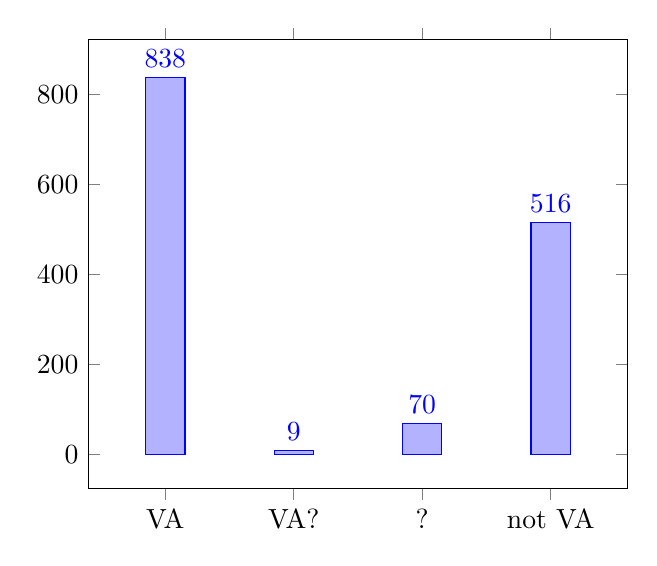
\begin{tikzpicture}
    \begin{axis}[ybar,nodes near coords, bar width=0.5cm,symbolic x coords={VA, VA?, ?, not VA},enlarge x limits=0.2]
    \addplot coordinates{ (VA,838) (VA?,9) (?,70) (not VA,516)};
    \end{axis}
    \end{tikzpicture}
\caption{Distribution of VA among the total of 1433 adjectives}
\label{fig:kamil:1}
\end{figure}

 With regard to which adjectives could derive Statives, the only semantic restriction found related to adjectives denoting ethnicities/geographic origins (e.g., \iwi{Akkad}{\textit{amurrû}} `Amorite', \iwi{Akkad}{\textit{elamû}} `Elamite', etc.). Perhaps owing to the contexts during which they are used being overwhelmingly of archival nature (i.e., inventory lists with items from said places), these adjectives were not found to derive Statives. 

All other adjective types derived at least one Stative, as shown in (\ref{ex:moresec}). Example (\ref{ex:moreseca}) shows a Stative from a participle, (\ref{ex:moresecb}) shows the Stative derived from a denominal adjective\is{denominal!adjective} derived with both \iwi{Akkad}{-\textit{ān}-} and \iwi{Akkad}{-\textit{ī}-}.

\begin{exe}  \ex More secondary Stative examples\is{derivation!stem-based}\label{ex:moresec}
\begin{xlist} \ex \label{ex:moreseca} \glll \iwi{Akkad}{\textit{šumma}} \textit{liqpî=šu} \textbf{\iwi{Akkad}{\textit{šābul}}}\\
    {} {} \iwi{Akkad}{${\surd}$\textit{ʔbl}}~`dry' \\
     if palate=his.\textsc{sg.m} \textsc{caus}.dry.\textsc{ptcp.stat.3sg.m}\\
    \glt `If his palate is dry (and covered with a deposit) ...' (\citetalias[ 64:54]{Labat_TDP})
  \ex \label{ex:moresecb} \gll \iwi{Akkad}{\textit{šumma}} \textit{imitt-a} \textit{tirk-u} \textbf{\iwi{Akkad}{\textit{lumnānî}}}\\
     if right-\textsc{obl} {dark.spot}-\textsc{nom} {evilly.inclined}.\textsc{stat.3sg.m}\\
    \glt `If there is a black spot on the right, he is prone to misfortune.' (\citetalias[ 29:14]{CT28})
    \end{xlist}    
\end{exe}

 As initially expected in Section \ref{sec:secstatsem} above, the vast majority of Statives appears in conditional \iwi{Akkad}{\textit{šumma}}-contexts. Further, the majority of Statives appears in the \textsc{3sg.m} form, i.e., they do not feature any Stative-suffixes. As they also lack case-marking, I exclude the possibility of predicatively used\is{predicative!usage} “regular” adjectives.

The attestation of (adjectival) secondary Statives\is{derivation!stem-based} is incredibly rare vis-à-vis the attestation of primary Statives.\is{derivation!deradical} As \citet{kraus_nominalsatze_1984} also noted in his study of the old Babylonian letters corpus (\textit{altbabylonische Briefe}), out of 1200 Statives attested in the selected volumes investigated, only 20 Statives were formed of nominal or adjectival stems, i.e., of secondary Statives.\is{derivation!stem-based} In my present study, comprising the attestations provided by the \textit{Chicago Assyrian Dictionary}, less than forty adjectives were found to certainly derive Stative forms.

From this statistical observation, I infer that the inheritance of a CoS event\is{change of state (CoS)} from the \textsc{root} is a necessity for Stative formation. Drawing a CoS \is{change of state (CoS)} from a pragmatic/modal context appears to have been more costly, and thus so rarely observed. This necessity to inherit eventive information from a \textsc{root} could also be argued to serve as further evidence for both the verbal, but particularly the \isi{resultative} nature of the state described by the Stative. We may now revise the schema in Table \ref{tab:Stativecategor4} for the last time.

\begin{table}
    \caption{Basic morphological Stative categorisation (final revision)}
\begin{tabularx}{\textwidth}{ c  c  c  c  c  c  c }
\lsptoprule
    \multicolumn{5}{ c}{Primary Statives\is{derivation!deradical}} & \multicolumn{2}{c}{Secondary Statives\is{derivation!stem-based}} \\
    \cmidrule(lr){1-5}\cmidrule(lr){6-7}
    \multicolumn{5}{ c }{\textit{XaY(i)Z}- + suffix} & \multicolumn{2}{c }{Stem + suffix} \\ \cmidrule(lr){1-4}\cmidrule(lr){5-5}\cmidrule(lr){6-7}
    \multicolumn{4}{ c }{Verbal \textsc{root}} & Adj.\ \textsc{root} & Adj.\ stem  & Nom.\ stem \\
    \cmidrule(lr){1-1}\cmidrule(lr){2-2}\cmidrule(lr){3-3}\cmidrule(lr){4-4}
    Unerg. & Unacc. & Agent.-tr. & Exp. & & \multicolumn{2}{c}{}  \\
    \cmidrule(lr){1-1}\cmidrule(lr){2-5}\cmidrule(lr){6-7}
    No Stat. & \multicolumn{4}{c }{Root-inherited CoS} & \multicolumn{2}{c}{External CoS event} \\ \lspbottomrule
\end{tabularx} 
    \label{tab:Stativecategor4}
% \begin{forest}for tree=forked edges, for tree={grow'=east}
%   [~,
%     [{Primary\\Statives}
%         [{{\textit{XaY(i)Z}-\\ + suffix}}
%             [Verbal \textsc{root}
%                 [Unergative
%                     [No Stat., no edge]
%                 ]
%                 [Unaccusative [, name=unacc, tier=brace, no edge]]
%                 [Agent-tr.
% %                     [Root-inherited CoS, no edge]
%                 ]
%                 [Exp, tier=leaf, name=exp]
%             ]
%             [Adj. \textsc{root}, tier=leaf [, name=adj, tier=brace, no edge]]
%         ]
%     ]
%     [{Secondary\\Statives}
%         [{Stem\\+suffix}
%             [Adj. stem, tier=leaf [,name=adjstem,tier=brace,no edge]
% %                 [External CoS event, no edge]
%             ]
%             [Nom. stem, tier=leaf [,name=nomstem,tier=brace,no edge]]
%         ]
%     ]
%   ]
% % \begin{tikzpicture}[overlay, remember picture]
% \draw[
%     decorate,
%     decoration={brace, amplitude=6pt}
% ]
% ([xshift=-18pt]unacc.north east) -- ([xshift=-18pt]adj.south east)
% node[midway, right=8pt]{Root-inherited CoS};
% \draw[
%     decorate,
%     decoration={brace, amplitude=6pt}
% ]
% ([xshift=-18pt]adjstem.north east) -- ([xshift=-18pt]nomstem.south east)
% node[midway, right=8pt]{External CoS event};
% \end{forest}
% \end{tikzpicture}

\end{table}
    

 I leave the question of diachrony open at this point, hypothesising that the \isi{resultative}/Stative attaching to adjectival or nominal stems potentially derived from parallel contexts of primary Statives\is{derivation!deradical} and adjectival/nominal stems in modal constructions, particularly in omens and medical texts. Given the scope of the present paper, this shall remain an endeavour for future studies to embark on.



\section{Conclusion}\label{sec:Akkconclusion}

This paper's goals were twofold: First, it set out to argue against the synchronic interpretation of all Statives as deadjectival verbs\is{deadjectival!verb} by presenting the allosemic Experiencer-subject alternation in primary Statives.\is{derivation!deradical}  This alternation could be accounted for by assuming that different functional heads, namely \textit{a} and \textit{v}, set different s-selectional requirements for the syntax to filter out the arguments necessary for their derivation. Ultimately, it shows that primary Statives\is{derivation!deradical} are not syntactically \is{deadjectival!verb}deadjectival.

Secondly, this paper sought to motivate the Stative's function as a \isi{resultative} state through cross-linguistic parallels of \isi{resultative} constructions. I argued that the referenced CoS \is{change of state (CoS)} event is implicitly encoded in the \textsc{root} of primary Statives.\is{derivation!deradical} The deadjectival \is{derivation!stem-based}secondary Statives,\is{deadjectival!verb} which lack eventive encoding, must draw their CoS \is{change of state (CoS)} context from external syntactic or semantic/pragmatic sources, most commonly from modal particles/complementisers. The Stative requiring access to eventive encoding could serve as further evidence for its \isi{resultative} function as well as an explanation for the scarcity of secondary Statives.\is{derivation!stem-based}

\section*{Acknowledgements}

For valuable comments and discussions relating to this article I would like to thank John Beavers,  Laura Grestenberger, Peter Hallman,  Pavel Iosad, Michael Jursa, Itamar Kastner, Andrew Koontz-Garboden, Dan Lassiter,  and Viktoria Reiter. I would also like to thank the two anonymous reviewers for their invaluable comments. All remaining shortcomings of this article remain mine alone.
 
 
\section*{Abbreviations}
\begin{tabularx}{.5\textwidth}{lQ}
    \textsc{acc} & accusative  \\
    \textsc{caus} & causative \\
    \textsc{com} & common gender  \\
    \textsc{conj} & conjunction  \\
    CoS & change of state  \\
    \textsc{cstr} & construct state  \\
    D & \emph{Dopplungstamm} / \textsc{intensive} pattern  \\
    \textsc{dat} & dative  \\
    DOR & direct-object restriction \\
    \textsc{f(em)} & feminine  \\
    G & \emph{Grundstamm} / \textsc{simple} pattern  \\
    \textsc{gen} & genitive  \\
    \textsc{ipfv} & imperfective \\
     IPP & independent personal pronouns\\
         \textsc{m(asc)} & masculine \\
\end{tabularx}
\begin{tabularx}{.47\textwidth}{lQ}
   \textsc{mod} & modal \\
     N & \emph{N-Stamm} / \textsc{passive} pattern \\
     \textsc{neg} & negation \\
   \textsc{nom} & nominative \\
  \textsc{obl} & oblique \\
     PC & property concept \\
     \textsc{pfv} & perfective \\
   PN & personal name \\
     \textsc{ptcp} & participle \\
     \textsc{pl} & plural \\
     RN & regnal name \\
    Š & \emph{Š-Stamm} / \textsc{causative} pattern \\
    \textsc{sg} & singular \\
     \textsc{stat} & Stative \\
    \textsc{tam} & tense/aspect/mood \\
    VA & verbal adjective \\
    \\
\end{tabularx}



{\sloppy\printbibliography[heading=subbibliography,notkeyword=this]}
\end{document}

